\documentclass[11pt, a4paper]{article}
\usepackage{fullpage}
\usepackage[utf8]{inputenc}
\usepackage[T1]{fontenc}
\usepackage{graphicx}
\usepackage{float}
\usepackage{tikz-uml}
\usepackage{amsmath}
\usepackage{amssymb}
\usepackage{listings}
\usepackage{hyperref}

\hypersetup{
    colorlinks=true,
    linkcolor=blue,
    filecolor=magenta,      
    urlcolor=cyan,
    bookmarks=true,
    pdfpagemode=FullScreen,
}

\newcommand{\besoinItem}[7]{
    \item #1
    \begin{description}
        \item[description :]
        #2 
        \item[priorité :]
        #3
        \item[faisabilité :]
        #4
        \item[références ou bibliothèques existantes :]
        #5
        \item[cas d'utilisation :]
        #6
        \item[test d'utilisation :]      
        #7 
    \end{description}
}
\newcommand{\besoinVItem}[5]{
	\item #1
	\begin{description}
		\item[description :]
		#2 
		\item[faisabilité: ]
		#3
		\item[cas d'utilisation :]
		#4
		\item[test d'utilisation :]      
		#5
	\end{description}
}

\newcommand{\besoinItemSimple}[4]{
	\item #1
	\begin{description}
		\item[description :]
		#2
		\item[cas d'utilisation :]
		#3
		\item[test d'utilisation :]      
		#4
	\end{description}
}

\title{Apprentissage par renforcement multi-agents, De SlimeVolley à la RoboCup : Cahier des besoins et d'essais/prototypes}
\author{Pélagie Alves\and Elias Debeyssac\and Alexis Hoffmann\and
Alexis Lhéritier\and Nicolas Majorel\and Sébastian Pagès}
\date{Février 2021}

\begin{document}

\maketitle

\newpage

\tableofcontents

\newpage

\section{Introduction}
Le projet << Apprentissage par renforcement multi-agents : de SlimeVolley à la RoboCup >> nous est proposé par Ludovic Hofer qui est membre de l’équipe Rhoban, un groupe de recherche en robotique du LaBRI. Cette équipe travaille notamment sur la robotique autonome et participe depuis presque 10 ans à la RoboCup. Notre client est spécialisé dans l’apprentissage par renforcement pour les robots.
\newline \newline
Dans le cadre de la RoboCup, les robots disputent des matchs de foot et sont donc amenés à prendre des décisions de manière autonome pour élaborer une stratégie. Pour cela on utilise l’apprentissage par renforcement dans un contexte multi-agents pour simuler des parties afin d'améliorer la prise de décision des robots sur le terrain.
\newline \newline
Notre objectif est de proposer une version simplifiée de la RoboCupSoccer pour faciliter l’apprentissage et l'évaluation de stratégies pour robots. Notre simulation devra être facilement paramétrable pour permettre de jongler entre différents environnements, c'est-à-dire qu'il faut pouvoir activer et désactiver certaines règles et options avant le lancement d'un match. 
En fonction de l'environnement dans lequel les robots d'une équipe auront été entrainés, ils vont développer une stratégie spécifique. Le but est de pouvoir observer l'efficacité de cette stratégie en la confrontant lors d'un match, à une autre provenant d'un autre environnement. Nous devons donc fournir un outil qui va permettre à l'utilisateur d'analyser et d'observer l'impact des modifications de règles et paramètres sur l'apprentissage des joueurs.
\newline \newline
Pour se familiariser avec l’apprentissage par renforcement dans un contexte multi-agents, notre client nous propose d’implémenter le mode deux contre deux dans le jeu SlimeVolleyBall et permettre d’apprendre des stratégies de deux contre deux en se basant sur le projet SlimeVolleyGym.
\newpage

\section{Description et Analyse de l'existant}

\subsection{RoboCup Soccer Humanoid League Laws of the Game 2019/2020}

Ce document \cite{robocuprules} répertorie toutes les règles et spécificités pour la compétition de Soccer de la RoboCup. 
Une première partie concerne la dimension du terrain de foot et les différentes zones de jeux. Il est composé de deux buts, deux zones de but, deux surfaces de réparation, deux moitiés de terrain et une zone d'engagement (cf Figure ~\ref{fig:ter}). 
On a principalement deux tailles de terrain : kid et adult, on peut retrouver les différentes dimensions ci-dessous (cf Figure ~\ref{fig:dim_ter}).
\newline
Les robots de la catégorie kid doivent mesurer entre 40cm et 100cm, ceux de la catégorie adult entre 100cm et 200cm. Tout robot doit avoir un BMI(Body Mass Indice) entre 5 et 30. Le BMI est le poids en kg du robot divisé par sa hauteur en $m^2$.
\newline
La balle doit être sphérique et a une taille différente en fonction des catégories. Pour la catégorie kidSize, la balle est une Fifa size 1 (circonférence=42cm, diamètre=13cm, poids 205g) et pour la catégorie adultSize, c'est une Fifa size 5 (circonférence=69cm, diamètre=22cm, poids 435g).
  \begin{figure}[H]
	\centering
	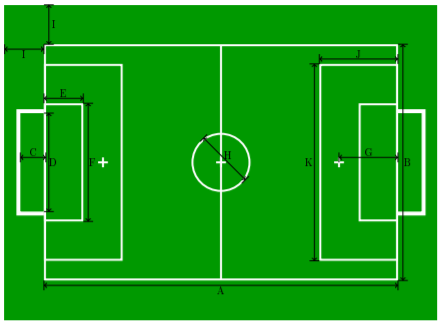
\includegraphics[scale=1.2]{images/ter.PNG}
	\caption {\cite{robocuprules}
		Schéma d'un terrain de foot pour la RoboCup}
	\label{fig:ter}
\end{figure}
\begin{figure}[H]
	\centering
	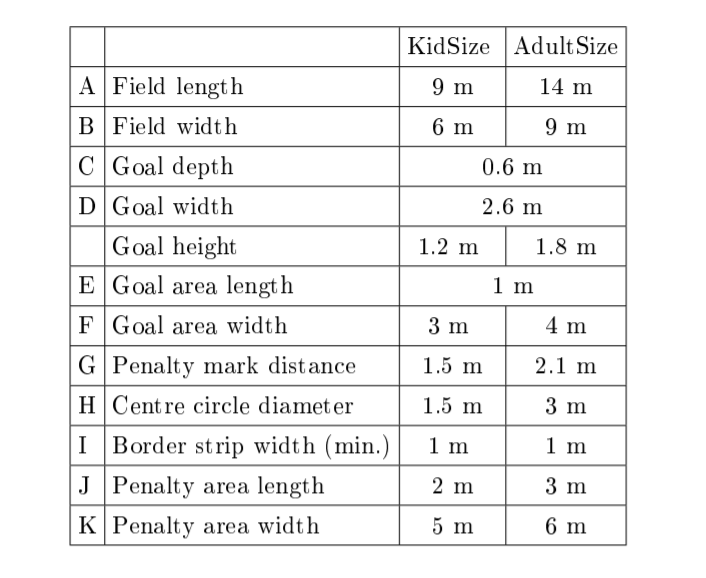
\includegraphics[scale=0.8]{images/dim_ter.PNG}
	\caption {\cite{robocuprules}
		Dimension du terrain de foot en fonction des catégories kidSize et adultSize}
	\label{fig:dim_ter}
\end{figure}
Le nombre de joueurs varie de 2 à 5 pour la kidSize et de 2 à 3 pour la version adultSize. Un des joueurs d'une équipe doit avoir le rôle gardien, il peut alors prendre la balle avec les mains mais doit rester dans la zone de but toute la partie.
\newline

Avant le début du match, les robots ont un maximum de 45s pour se positionner, chaque équipe doit être dans sa moitié de terrain. La balle est positionnée au centre, les joueurs adverses doivent être à au moins 0.75m de la balle en kidSize et 1.5m en adultSize. Si un joueur est mal placé, il est sorti le temps du lancement du match. Le match est lancé dès que la balle est en mouvement ou que 10s se sont écoulées.
\newline
Lorsqu'un but est marqué, l'équipe qui a encaissé le but procède à l'engagement au centre du terrain. L'équipe qui a marqué gagne un point. Si une équipe marque contre son camp, le but n'est pas comptabilisé mais l'équipe adverse obtient un corner.\newline

Le match est décomposé en 2 mi-temps de 5 min s'il n'y a pas de gagnant à la fin, on peut procéder à des tirs au but.\newline

Si une faute est commise, le joueur en tort peut être exclu 30s (surtout s'il fait perdre du temps durant le match). Le joueur exclu attend à une position bien spécifique jusqu'à que l'arbitre l'autorise à revenir en jeu.\newline

Si un joueur prend la balle avec ses mains (à part le gardien), bloque un adversaire ou entre en collision avec lui, un coup-franc est donné pour l'équipe adverse.
Si une telle faute est commise sur la surface de réparation, il y a penalty.

Lorsqu'un joueur sort la balle, il y a une touche pour l'équipe adverse (possibilité de prendre la balle avec les mains pour faire la touche), si la balle est sortie sur la ligne de but de l'équipe A par l'équipe A, alors l'autre équipe obtient un corner.

\subsection{Environnement de développement}



Le projet sera programmé en python et utilisera les bibliothèques Numpy\cite{numpy}, Gym\cite{openaigym} et stable-baselines\cite{stable-baselines}. 
Numpy permettra de gérer des tableaux et des matrices. Gym permettra de créer un modèle pour développer et comparer des algorithmes d'apprentissage par renforcement.
Gym nous permettra de créer et manipuler des environnements \cite{openaigymGit} (on définira par la suite ce terme en prenant comme exemple SlimeVolleyBall). Stable-baselines permet d'utiliser 
des algorithmes d'apprentissage par renforcement 
(comme PPO\cite{PPO} utilisé dans slimevolleygym\cite{slimevolleygym}) pour récupérer des comportements à adopter en fonction des environnements. Le fonctionnement interne des algorithmes implémentés dans stable-baselines ne nous intéresse pas, 
car nous nous contenterons de les utiliser.



\subsection{SlimeVolleyGym}
\subsubsection{Présentation}
SlimeVolley est un jeu apparu pour la première fois en juin 1999. Le principe est simple, deux slimes en forme de demi-cercle s'affrontent dans un  match de volley. Dans la version standard, un slime est contrôlé par un humain et l’autre est contrôlé par l’ordinateur mais il est aussi possible que deux personnes jouent sur le même clavier en local. Chaque slime dispose de trois touches directionnelles. La flèche du haut pour sauter, la droite et la gauche pour respectivement se déplacer à droite et à gauche. Le terrain de jeu est divisé en deux parties par un filet de la taille d’un slime. Chaque slime a pour but de frapper la balle avec son corps en prenant en compte les intéractions physiques du jeu pour la faire tomber sur le sol de l’adversaire. Chaque Slime à 5 vies, une fois que la balle touche le sol d’un joueur, alors une vie est enlevée à celui-ci. La partie se termine quand un joueur atteint 0 vie. Il a alors perdu. Il est également impossible au slime de “sauter” par dessus le filet pour aller sur le terrain adverse.  \\
La version Python que nous utilisons dans ce projet est l’adaptation d’une version de 2015 en Javascript. Elle est développer avec la bibliothèque Gym qui est un environnement d'entraînement d'intelligence artificielle utilisant l’apprentissage par renforcement. SlimeVolleyGym est un projet d'apprentissage par renforcement développé par David Ha\cite{slimevolleygym},nous expliquerons ce concept dans le paragraphe suivant.

\subsubsection{Apprentissage par renforcement}
L'apprentissage par renforcement est une méthode d'apprentissage qui consiste a récompenser ou punir les agents (entités autonomes) en fonction des actions qu'ils accomplissent. L'idée est de laisser l'agent apprendre de ses erreurs. Par exemple, si on pénalise l'agent pour  un certain comportement, il peut renoncer à celui-ci, si on le récompense cela va au contraire l'encourager à le reproduire.

Dans l'apprentissage par renforcement,on a un agent et un environnement. L'environnement est le modèle dans lequel évolue les agents à un instant donné, il prend également en compte l'observation de l'agent c'est-à-dire ce que l'agent perçoit du modèle. La récompense que l'agent reçoit fait également partie de l'environnement. Ce nombre est un indicateur de l'évaluation du comportement de l'agent pou un environnement donné. L'objectif de l'agent est de maximiser son score de récompense c'est pour cela qu'il répète des comportements juger positifs par l'environnement et élabore une stratégie adaptée à celui-ci.


\subsubsection{Processus décisionnels de Markov}

On illustre souvent les concepts fondamentaux de l'apprentissage par renforcement avec le formalisme mathématique suivant : \\

\noindent $\left\langle \mathbf{S}, \mathbf{A}, \mathbf{T}, R, P\right\rangle $\\ \\
$\mathbf{S} :$ est l’espace d’états dans lequel évolue le processus \\
$\mathbf{A} :$ est l’espace des actions qui contrôlent la dynamique de l’état  \\ 
$\mathbf{T} :$ est l’espace des temps, ou axe temporel\\
$P :$ est la fonction de probabilité de transition entre les états $s_t$ et $s_{t+1}$ en executant l'action a : $\mathcal{P} \left(s_{t+1}|s_t,a\right)$ \\	
$R : \mathbf{S} \times \mathbf{A} \times \mathbf{S} \rightarrow \mathbb{R} $, la fonction de récompense, avec $r_t = \mathbf{R}\left(s_t, a_t, s_{t+1}\right)$  \\
\\

\noindent Tous les états ont la propriété «Markov», faisant référence au fait que l'avenir ne dépend que de l'état actuel.

\noindent \textbf{S} : L'état est la description complète de l'environnement à un instant t comme si on mettait le jeu en pause. \\
Dans SlimeVolley l'état comprend différents éléments comme la taille du terrain, la position et la taille du filet, la position de la balle, sa hitbox, sa vitesse, la direction dans laquelle elle va, les agents : leur position et leur espace d'observation (voir Représentation de l'environnement SlimeVolleyBall pour plus de détail). L'espace d'observation peut varier de partiel à complet. \\

\noindent \textbf{A} : L'espace d'action représente toutes les possibilités d'actions pour l'agent dans le modèle. Dans le cadre de SlimeVolley il s'agit seulement de mouvements : droite, gauche, haut. Il peut arriver que ces déplacements soient contraints par exemple l'agent ne doit pas sortir de sa moitié de terrain, si on accède à un déplacement non autorisé, alors il n'est pas appliqué.\\

\noindent \textbf{R} : La récompense est attribuée à l'agent en fonction de ses actions. Pour SlimeVolley, si l'agent marque un point alors il reçoit +1 en récompense en revanche s'il rate la balle et la laisse tomber il reçoit -1. \\\\

\begin{figure}[H]
	\centering
	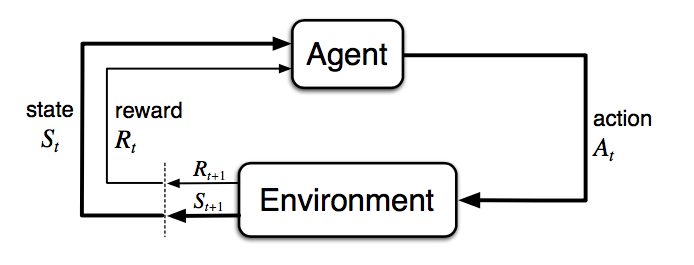
\includegraphics[scale=0.5]{images/agent_environment_MDP.png}
	\caption {Schéma du processus décisionnel de Markov \cite{openaigym}}
\end{figure}


\noindent Pour de plus amples informations sur la représentation d'un environnement avec Gym, il faut se diriger vers l'annexe \href{/annexes/Environnement_SlimeVolleyBall.pdf}{Environnement SlimeVolleyBall}.


\subsubsection{Fonctionnalités de SlimeVolleyGym}
SlimeVolleyGym permet de créer des environnements de jeu et de simuler des parties en intégrant des algorithmes d'apprentissage par renforcement. Ces algorithmes pourront ainsi s’entraîner et s'évaluer en jouant contre eux-mêmes ou contre d'autres algorithmes déjà implémentés dans SlimeVolleyGym. Un mode Humain contre Humain et Humain contre Machine sont également implémentés. \\ \\

Il y a trois façons d'utiliser SlimeVolleyGym. La première consiste à entraîner un algorithme déjà existant ou créé par l'utilisateur. Des exemples d'algorithmes sont déjà implémenté par l'auteur dans le répertoire training-script.
La seconde permet d'évaluer un algorithme en le faisant jouer contre une autre. Les fichiers pour évaluer un algorithme sont :eval\_agent.py, eval\_ppo.py et eval\_ppo\_pixel. Plusieurs paramètres sont disponibles pour lancer un entraînement, ils seront explicités au point suivant.
La dernière façon consiste à utiliser les fichiers test\_state.py, test\_pixel.py et test\_atari.py pour faire jouer un humain contre un algorithme déjà implémenté par l'auteur ou faire une partie Humain contre Humain. Chaque joueur humain pourra choisir son "camp" en jouant soit avec les touches W, A, S, D (côté gauche) ou avec les flèches directionnelles (UP, DOWN, RIGHT, LEFT) (côté droit).\\ \\

SlimeVolleyGym implémente déjà plusieurs paramètres ainsi que deux environnements (SlimeVolley-v0 et SlimeVolleyNoFrameskip-v0). Les paramètres disponibles pour les fichiers d'évaluations sont : 

Pour le fichier eval\_agents.py :
\begin{itemize}
\item - -left <baseline/cma/ppo/ga/random> : Permet d'affecter un algorithme choisi sur la partie gauche de la fenêtre de jeu.
\item - -right : <baseline/cma/ppo/ga/random> : Permet d'affecter un algorithme choisi sur la partie droite de la fenêtre de jeu
\item - -leftpath : Permet d'affecter un algorithme à gauche en spécifiant son chemin et répertoire. Laisser vide pour utiliser les algorithmes déjà implémentés dans le répertoire zoo.
\item - -rightpath : Permet d'affecter un algorithme à droite en spécifiant son chemin et répertoire. Laisser vide pour utiliser les algorithmes déjà implémentés dans le répertoire zoo.
\item - -render : Active le rendu graphique du jeu.
\item - -day : Change la couleur du jeu en la mettant en version "jour"(Claire). Par défaut, la version "nuit"(Sombre) est activée(Sombre). 
\item - -pixel : Active le mode d'affichage "pixel"
\item - -seed <...> : Permet de choisir la graine aléatoire de la partie. Laisser vide pour générer la graine aléatoire.
\item - -trials : Permet de choisir le nombre de parties que vont jouer les algorithmes. Par défaut, la valeur est de 1000.
\end{itemize}

Pour le fichier eval\_ppo.py :
\begin{itemize}
\item - -model-path <...> : Chemin vers le modèle voulant être utilisé. 
\item - -render : Pareil que le paramètre render déjà défini.
\end{itemize}

Pour le fichier eval\_ppo\_pixel.py :
\begin{itemize}
\item - -model-path <...> : Pareil que le paramètre model-path déjà défini.
\item - -seed <...> : Pareil que le paramètre seed déjà défini.
\end{itemize}

Le diagramme de cas d'utilisation de SlimeVolleyGym peut être défini comme cela.
 \begin{figure}[H]
    \centering
    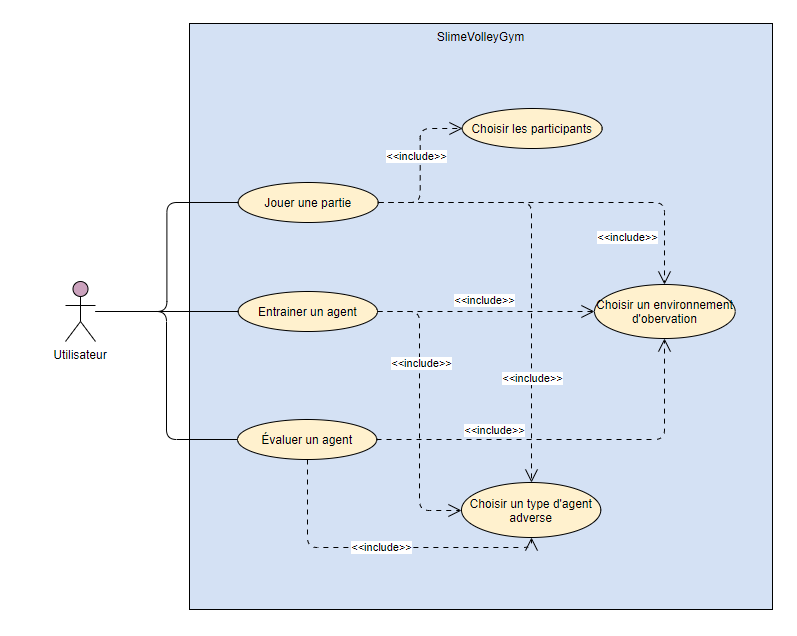
\includegraphics[scale=0.7]{images/cas_utilisation.PNG}
    \caption {Diagramme de cas d'utilisation de SlimeVolleyGym}
\end{figure}


Voici comme exemple, un diagramme de séquence lors du lancement d'une partie en mode Humain contre Machine.
 \begin{figure}[H]
    \centering
    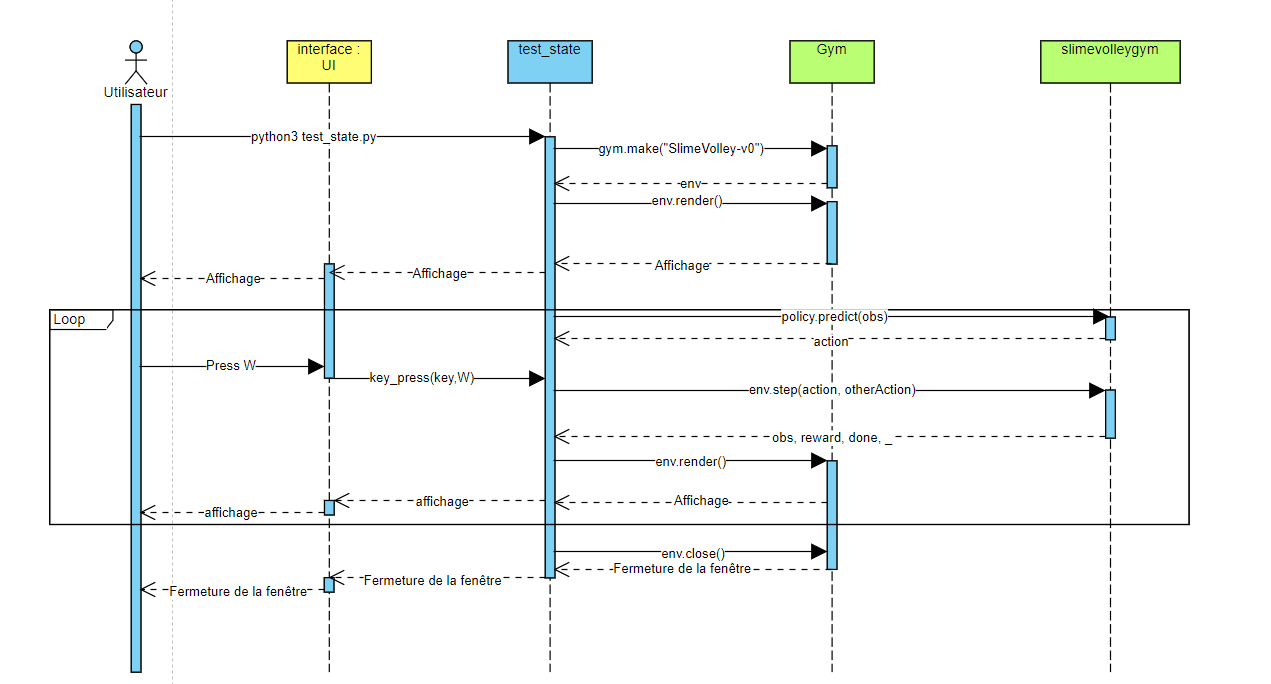
\includegraphics[scale=0.5]{images/diagramme_sequence.PNG}
    \caption {Diagramme de séquence lors de l’exécution du fichier test\_state.py en mode Humain contre Machine}
\end{figure}
\hypertarget{link2}{\subsubsection{Architecture}}
L'architecture déjà existante de SlimeVolleyGym se présente comme ceci :
\begin{figure}[H]
    \centering
    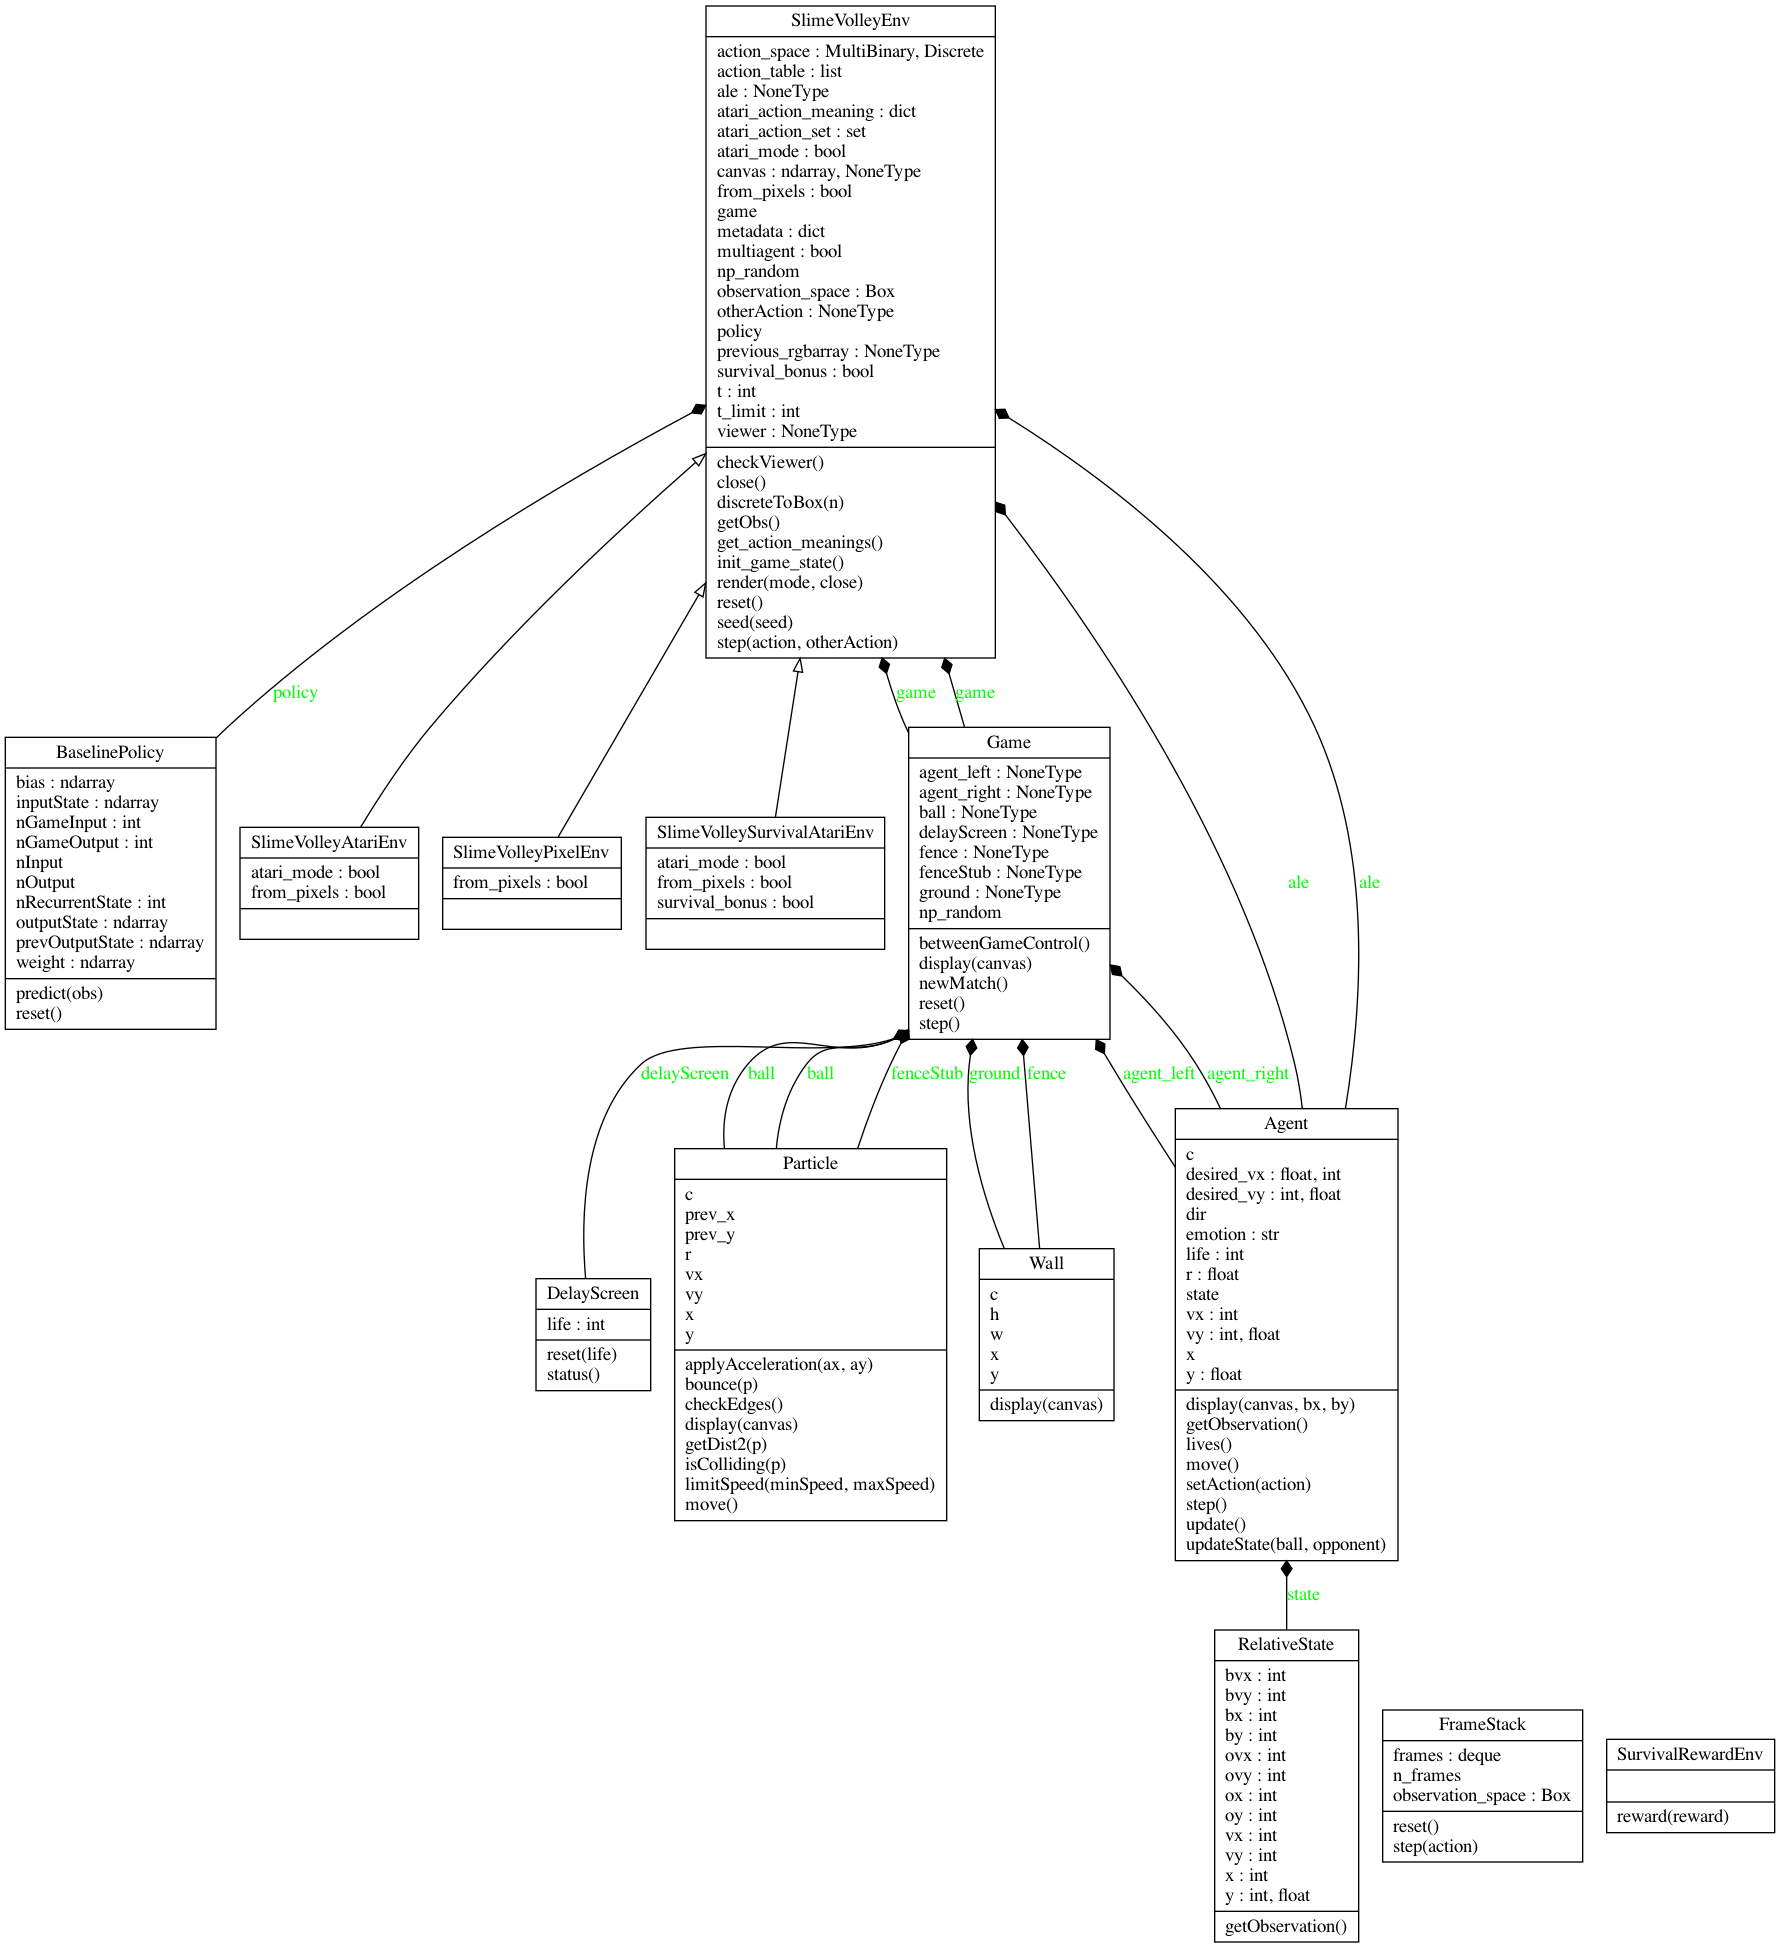
\includegraphics[scale=0.25]{images/classes.png}
    \caption {Diagramme de classes du fichier SlimeVolleyGym.py}
\end{figure}


Tout d'abord, on a les classes fondamentales qui définissent comment sont construits les différents éléments dans le jeu comme les agents(joueurs), la balle, les états, la fenêtre(affichage et rafraîchissement). \\

\begin{itemize}
\item Particle : Permet de définir la balle et ses différentes actions (affichage, déplacement, test de collision, rebond et vitesse max). Cette classe prend en entrée la position x et y de la balle, ses vecteurs de vitesse vx et vy, son rayon r et sa couleur c.\\

 \item Wall : Permet de définir le mur séparant les deux joueurs et le sol sur lequel les joueurs se déplacent. Les valeurs d'entrées nécessaires sont la position en x et y, sa longueur w, sa hauteur h et sa couleur c.\\

 \item Agent : Définit un agent(un joueur) et les actions qu'il va effectuer (sauter, se déplacer). L'agent prend en entrée sa position x et y, une couleur c et sa position sur le terrain (côté droit(1) ou côté gauche(-1)).\\

\end{itemize}
Les trois classes présentées ci-dessus renvoient un objet Canvas après sa création qui permettra d'être affiché sur la fenêtre de jeu. \\
\begin{itemize}
 \item RelativeState : Sauvegarde l'état précédent et actuel du point de vue d'un agent. La classe est utilisée par la classe Agent pour garder une trace de l'état du jeu après chaque action. Les éléments sauvegardées dans l'état sont, la position et le vecteur vitesse de l'agent lui-même, de son adversaire et de la balle. Ces valeurs sont stockées dans une matrice de taille $3 \times 4$. Avec chaque ligne correspondant aux valeurs de l'agent pour la première, de la balle pour la seconde et enfin de son adversaire.

 \item DelayScreen : Bloque la balle pendant 30 rafraîchissements d'image avant chaque remise en jeu. La valeur peut être modifiée avec la variable globale INIT\_DELAY\_FRAMES.\\

\end{itemize}

Ensuite les classes de jeu, correspondant aux classes qui ont pour but de créer l' environnement, de définir les modes de jeu (Atari ou Pixel) et de créer un algorithme d'apprentissage par renforcement (BaselinePolicy). Elles sont définies par les classes : \\
\begin{itemize}
 \item SlimevolleyEnv : SlimeVolleyEnv implémente l'interface Env de la librairie Gym. C'est avec cette classe, que les actions possibles sont définies (Droite, gauche et sauter) mais également les modes de jeu Atari, Pixel et Survival. Cette classe définit également, la façon dont les récompenses sont distribuées (score général, score en fonction du temps où la balle n'a pas touché le sol ou la somme des deux précédents).\\

 \item BaselinePolicy : BaselinePolicy intègre un petit réseau de neurones récurrents(annotation) appelé par la classe SlimeVolleyEnv et pouvant être utilisé par défaut dans un entraînement.\\

 \item SlimeVolleyPixelEnv : Mode de jeu pré-configuré pour l'environnement. Le jeux est alors pixelisé et il y a moins d'images par seconde. Le mode Pixel(faire une annotation) est activé. \\
 
 \item SlimeVolleyAtariEnv : Mode de jeu pré-configuré pour l'environnement. Il permet de montrer le fonctionnement du pré-traitement des images qui seront empilées dans le mode pixel. Le mode Atari(faire une annotation) est activé. \\ 

\item SurvivalRewardEnv : Mode de jeu pré-configuré pour l'environnement. Le mode Survival récompense l'agent en fonction de son temps de survie. Plus l'agent ne fait pas tomber la balle sur le sol, plus il est récompensé. La classe SurvivalRewardEnv prend un environnement en entrée.
 \item  SlimeVolleySurvivalAtariEnv : Mode de jeu pré-configuré pour l'environnement. Les trois modes préalablement définis sont activés. \\

 \item Game : Cette classe gère l'initialisation de la partie, affiche les éléments à l'écran, lance un match ou le recommence, gère le nombre de vies restantes par agent et s'il a gagné ou perdu. Elle contient également la boucle de jeu qui à chaque étape, gère les déplacements des agents et de la balle, vérifie qu'il y a une collision et actualise les états de chaque Agent. Elle prend en entrée un nombre aléatoire qui sera la graine de jeu de la partie. 

\end{itemize}

Et enfin, la classe FrameStack. Cette dernière prend en entrée un environnement de jeu et un nombre d'images à stocker. Elle utilise également la classe importée de la librairie Gym Wrapper. Wrapper permet d'ajouter des fonctionnalités à un environnement comme par exemple, la méthode de récompense des agents. FrameStack permet de traiter les actions provenant du clavier lors d'appui sur les touches W,A,S,D ou UP, DOWN, RIGHT, LEFT (flèches directionnelles) et d'envoyer à chaque Agent l'action du clavier ou celle prédit par sa méthode d'apprentissage.


\section{Analyse des besoins}
On décrira la liste des besoins fonctionnels et non-fonctionnels relatifs à l'implémentation du multi-agents dans Slime Volley Gym et la simulation de la RoboCup ci-dessous. On donnera des niveaux de priorité à ces besoins selon la classification suivante : 
\begin{itemize}
\item \textit{Mandatory} : les besoins obligatoires et nécessaires au bon fonctionnement de l'application.
\item \textit{Important} : les besoins qu'il serait important d'implémenter afin de rendre l'application intéressante. 
\item \textit{Optional} : les besoins optionnels qui permettraient d'enrichir l'application et de la rendre plus paramétrable.
\end{itemize}


\subsection{Besoins communs entre SlimeVolleyGym et la Robocup}
\begin{enumerate}
\besoinItem{input du JSON}
{Le but de notre projet est de permettre à OpenAI Gym de récupérer des instructions pour initialiser
une partie avec des paramètres spécifiques. Et pour cela, on va les lui donner à l'aide d'un fichier JSON.
Il fera office de fichier de configuration.
Il contiendra les options de l'environment de la partie que l'on veut lancer.}
{\textit{Mandatory}}
{JSON (JavaScript Object Notation - Notation Objet issue de JavaScript) est un format léger 
d'échange de données. Il est facile à lire ou à écrire pour des humains. 
Il est aisément analysable ou générable par des machines.}
{Pour écrire dans le JSON, on pourra utiliser la librairie argparse.py\cite{argparse.py} et json.py\cite{json.py} 
ou écrire directement dans le fichier.}
{Pour lancer une partie dans un environnement voulu, on peut modifier auparavant le fichier .json puis le passer en argument. On peut par exemple, changer la taille du terrain, mettre le champ $'collision': true$ pour autoriser les collisions entre agents, ... .}
{Test 1 : Après lancement d'une commande avec ArgParse, on vérifie bien que les champs correspondant aux arguments dans le fichier ont étaient modifiés.\\
 Test 2 : On modifie "à la main" le fichier JSON. On lance une partie en appelant ce fichier puis on vérifie que le fichier peut être lu par python sans faire remonter d'erreur.}

\besoinItem{Lecture du JSON et initialisation}
{Maintenant, pour pouvoir lancer la partie, il faut lire les informations contenus
dans le JSON et que le programme puisse les utiliser correctement.}
{\textit{Mandatory}}
{La lecture et l'interprétation de fichier JSON en Python à était reprise dans beaucoup de projet et des tutoriaux sont disponibles librement\cite{Tuto-JSON}. }
{Il existe la librairie json.py\cite{json.py} en python à importer.}
{Apres parsing du fichier JSON, la fonction d'initialisation de la partie va utiliser les données novuellement modifié pour lancer la partie avec par exemple l'activation ou non de la méthode qui vérifie que deux agents sont en collision.}
{On lance une partie avec le fichier JSON en paramètre. Puis on regarde si la partie s'exécute bien avec les mêmes entrées que dans le fichier JSON.}

\besoinItem{outputs en CSV}
{Concernant la gestion des ouputs, lorsque l'on décide de générer un fichier 
avec le résultat de tous les matchs, on va obtenir un fichier CSV.}
{\textit{Mandatory}}
{Comma-separated values, connu sous le sigle CSV, est un format texte ouvert
représentant des données tabulaires sous forme de valeurs séparées par des virgules.}
{La libraire csv.py\cite{csv.py} est adaptée pour ce besoin.}
{Après 10 matchs de 5 IA différentes, dans notre fichier csv, on pourra observer un tableau de 5x5 
avec le résultat dans la case correspondante à l'affrontement de 2 IA.}
{Après la fin de chaque match, on vérifie si l'issue d'un match correspond bien avec l'output contenu dans le fichier csv.}

\end{enumerate}

\subsection{Besoins fonctionnels pour l'extension de SlimeVolleyGym}


 
\begin{itemize}
\item \textbf {Définir un environnement avec 4 agents, 2 par équipe (environnement principal)}            \textit{(Mandatory)}

\begin{enumerate}
		
  \besoinVItem{\hypertarget{link3}{Définir l'espace d'observations}}
  {On souhaite définir l'espace d'observations pour pouvoir récupérer des informations sur l'état de l'environment.}
  {Pour définir le nouvel espace d'observations, on s'appuiera sur le code de SlimeVolleyBall, voir l'annexe \href{/annexes/Environnement_SlimeVolleyBall.pdf}{Environnement SlimeVolleyBall}, partie \textbf{2.3}. Il n'est pas nécessaire à priori de modifier l'espace d'observations par pixels. Il faut seulement modifier
  l'espace d'observations par états.  L'intervalle de valeurs acceptées est identique, on utilisera également l'objet Box pour représenter l'espace (Space) .

  $$
  \begin{bmatrix}
      x\_agent1 & y\_agent1 & \dot{x} \_agent1 & \dot{y}\_agent1 \\
      x\_ball & y\_ball & \dot{x}\_ball & \dot{y}\_ball \\
      x\_agent2 & y\_agent2 & \dot{x} \_agent2 & \dot{y}\_agent2 \\
      x\_agent3 & y\_agent3 & \dot{x} \_agent3 & \dot{y}\_agent3 \\
      x\_agent4 & y\_agent4 & \dot{x} \_agent4 & \dot{y}\_agent4 \\
  \end{bmatrix}
  \quad
  $$}
  {Pour tester que chaque Agent est indépendant, nous pouvons créer une simple test qui modifiera de manière aléatoire les valeurs de chaque Agent. Nous pourrons alors vérifier que chaque ligne du tableau qui représente les agents est bien indépendante.}

	\besoinVItem{Ajouter les deux nouveaux agents dans l'environnement}
	{ 
		On souhaite ajouter les deux nouveaux agents dans l'environnement, pour ce faire il faut procéder de cette manière : \\
		Créer deux agents, en suivant le même modèle de création que les deux agents précédents, il faudra seulement modifier la position de départ des agents de chaque "équipe" 
		pour qu'ils soient suffisamment espacés.
		
	}
	{
		On s'appuiera sur la classe \hyperlink{link2}{\textbf{Game}}, pour observer comment les agents sont créés dans le jeu. \\
		On utilisera également le même type de classe pour instancier un objet Agent (classe \hyperlink{link2}{\textbf{Agent}}).
	}
	{
		Lorsque l'agent est créé lors de l'initialisation, la boucle principale de jeu va modifier l'espace d'observation et ajouter les valeurs de base de l'agent. Ces données seront utilisées plus tard pour la collision de l'agent avec l'environnement ou encore plus tard avec son autre allié sur le terrain. Ces valeurs seront aussi utilisées par l'algorithme d'apprentissage par renforcement pour se créer un comportement en fonction de la position et la vitesse de chaque Agent.
	}
	{
		Nous allons vérifier que la liaison entre l'objet et l'espace d'observation fonctionne bien en modifiant aléatoirement la position et la vitesse de l'agent. 	
	} 
	

  \besoinVItem{Mettre à jour l'état relatif pour chaque agent}
	{ 
		En conséquence de l'ajout des deux nouveaux agents, il faut mettre à jour l'état relatif de chaque agent, pour rappel, ces données d'observations sont renvoyées par l'environnement
		dans le mode d'\textbf{observation par états} (voir l'annexe \href{/annexes/Environnement_SlimeVolleyBall.pdf}{Environnement SlimeVolleyBall}, partie \textbf{2.3}).\\
		Il faudra donc avoir pour chacun des agents des informations relatives (vitesse, position) sur les trois autres agents et sur la balle.
	}
	{
  		Il faudra adapter la classe \hyperlink{link2}{\textbf{RelativeState}} pour prendre en compte les informations sur les deux nouveaux agents.

	}
	{
        Lorsqu'un utilisateur ou un algorithme envoie une action sur l'agent nouvellement créé, celui-ci va se déplacer dans la direction souhaitée.L'espace d'observation sera alors modifié.
	}
	{
		Pour tester que l'espace d'observation est modifié de manière rationnelle, nous pouvons transmettre les mêmes actions que fait l'Agent allié à l'Agent nouvellement créé. Si les déplacements ainsi que la modification de l'espace d'observation ne sont identiques alors, il y a un problème de modification de l'espace d'observation.
	}


	\besoinVItem{Afficher les deux nouveaux agents dans l'environnement}
	{ 
		On souhaite afficher les deux nouveaux agents dans l'environment, l'affichage doit être différent selon le mode d'observation (états, pixels).
	}
	{
		Il suffira d'adapter la méthode \textbf{display(self, canvas)} de la classe \hyperlink{link2}{\textbf{Game}} pour permettre l'affichage des deux nouveaux agents. \\
		Comme spécifier dans l'annexe \href{/annexes/Environnement_SlimeVolleyBall.pdf}{Environnement SlimeVolleyBall}, partie \textbf{2.5}, le code de base permet déjà de 
		créer plusieurs types de forme géométrique en fonction du mode d'observation. \\ Dans notre cas, il est nécessaire de représenter et d'afficher des demis-cercle, on
		peut réutiliser la fonction \textbf{display(self, canvas, bx, by)} de la classe \hyperlink{link2}{\textbf{Agent}} qui se contente de modifier le canvas passé en paramètre en rajoutant 
		le demi-cercle représentant l'agent (en fonction de ses coordonnées, de son rayon, de sa couleur), mais également d'autres petits cercles pour afficher les yeux. Les yeux fixent la balle, 
		en s'appuyant sur les coordonnées bx et by fournies en paramètre.  \\
	}
	{
		Après l'initialisation de l'environnement avec les nouveaux \textbf{display(self, canvas, bx, by)} ajouté, la fenêtre (paramètre --render) va afficher tout les Agents en plus des éléments du terrain. Après chaque action puis chaque actualisation du canvas, les différents agents se déplace sur la fenêtre.
	}
	{
		Pour tester que l'affichage est valide, nous pouvons comparer la position des Agents dans l'espace d'observation et l'affichage sur la fenêtre. 
	} 

	\besoinVItem{\hypertarget{link1}{Gérer les collisions entre les agents de la même "équipe"}}
	{ 
		Pour que les agents ne se traversent pas, on ne va pas simplement délimiter le périmètre des agents dans chaque partie du terrain, car on ne souhaite pas limiter le champ d'action des agents \\
		, on préfère que ceux-ci apprennent des suites de l'entraînement des comportements positifs, par exemple qu'ils apprennent à bien s'espacer pour bien occuper les parties du terrain et donc optimiser le rattrapage 
		de la balle. \\
		Il faut pour cela gérer les collisions entre les agents de la même équipe, ils ne doivent pas non plus passer par en dessous, au-dessus l'un à l'autre.
				
	}
	{
		On pourra simplement définir que si la distance en x entre les deux slimes est inférieure à la somme des rayons des slimes il y a donc une collision. 
		Cela ne fera pas très propre visuellement, mais cela règle les deux problèmes cités au-dessus.

	}
	{
        Lors d'une partie normale, un joueur pourra rentrer en collision avec son allié. De même que pour le sol ou le mur séparant les deux équipes, chaque joueur ne pourra pas "traverser" son allié.  À part si l'un des Agents "saute" au-dessus de son allié.
	}
	{
        En pleine partie nous pouvons dire à chaque Agent de se déplacer vers le mur. Si l'Agent le plus éloigné ne "traverse" pas son allié, alors la fonction est validée.
		Nous pouvons aussi tester de sauter au-dessus de l'autre Agent pour vérifier qu'en cas de collision par le haut ou le bas, les Agents ne se "traversent" pas.
	} 

	\besoinVItem{Modifier le système de récompenses pour récompenser ou punir les agents de la même "équipe", la collision entre deux agents de la même équipe n'entraîne pas de pénalité}
	{ 
  		Il faut adapter le système de récompenses de SlimeVolleyBall pour récompenser ou punir les agents de la même équipe, dans cet environnement la collision entre deux agents de la même équipe 
		  n'entraîne pas de pénalité donc les règles sont identiques au SlimeVolleyBall de base.
	}
	{
		On pourra créer une classe \textbf{Team} avec pour attributs deux agents de la classe \hyperlink{link2}{\textbf{Agent}}, depuis cette classe, on synchronisera le résultat des deux agents de la même équipe, il ne sera pas 
		nécessaire de modifier la classe \textbf{Agent}. On pourra réutiliser la même fonction \textbf{checkEdges(self)} de la classe \textbf{Particle} (pour la balle) qui retourne 1 si la balle a touchée le sol du terrain de droite, 
		-1 si elle a touché le sol du terrain de gauche, 0 si elle est encore en jeu. Dans l'annexe \href{/annexes/Environnement_SlimeVolleyBall.pdf}{Environnement SlimeVolleyBall}, partie \textbf{2.6}, on spécifie 
		que la classe \textbf{Game} renvoie le résultat de l'action selon la perspective de l'agent de droite, cette-ci fois ce sera donc \underline{selon la perspective de l'équipe de droite}. \\
  
	}
	{
        Lors d'une partie, chaque algorithme d'apprentissage par renforcement se voit attribuer une récompense ou un malus en fonction de ses actions. C'est avec ce système que les algorithmes apprennent au fil du temps. 
	}
	{
        Pour tester que le système prend bien en compte la collision entre deux Agents, nous pouvons afficher dans la console la phrase "Collision effectué" lorsqu'une collision a lieu entre les agents.
	} 

\end{enumerate}

\item \textbf {Définir un sous-environnement dans lequel la collision entre 2 agents de la même équipe entraîne une pénalité (environnement fils)} \textit{(Important)}
\begin{enumerate}
	\besoinVItem{Modifier le système de récompenses pour récompenser ou punir les agents de la même "équipe", la collision entre deux agents de la même équipe entraîne une pénalité}
	{ 
		À la suite de l'implémentation de la \hyperlink{link1}{\textbf{collision pour les deux agents de la même équipe}}, il sera nécessaire de modifier le système de récompenses pour récompenser
		 	punir des agents de la même équipe après une collision. En conséquence de cela, on espère pouvoir observer des comportements intéressants :

		\begin{itemize}
			\item Conséquences positives : les deux agents apprennent à bien s'espacer et donc à optimiser le rattrapage de la balle
			\item Conséquences négatives : les deux agents apprennent à s'éviter totalement quitte à laisser tomber la balle
		\end{itemize}

	}
	{

		En cas de collision entre deux agents de la même équipe, on pourra opérer de manière drastique en attribuant un point à l'équipe adverse. Ou en enlevant un point à notre équipe directement dans le score global de la partie.

	}
	{
        Pendant une partie, les deux Agents vont devoir faire un choix sur qui doit aller récupérer la balle quand celle-là va tomber entre les deux Agents. Car si une collision a lieu, un malus d'un point pour l'équipe sera appliqué. Le comportement ainsi obtenu sera intéressant à observer et à évaluer dans d'autres environnements.
	}
	{
        Comme pour le test précédent, une fois une collision effectuée entre deux Agents alliés, on soustrait un point à l'équipe. Nous pouvons donc vérifier que le score total de l'équipe à bien diminuer et que l'affichage est bien actualisé.
	} 
\end{enumerate}





\item \textbf {Définir un sous-environnement dans lequel la largeur du terrain peut être modifiée (environnement fils)} \textit{(Important)}

\begin{enumerate}

	\besoinVItem{Définir l'espace d'observations}
	{ 

		De la même manière que le définition de l'espace d'observations pour l'\hyperlink{link3}{\textbf{environnement principal}}, il va être nécessaire de modifier l'espace d'obervations en conséquence de l'augmentation
		de la taille du terrain.

	}
	{

		On utilisera le même espace d'\textit{observation par états} que l'\textit{environnement principal}, cependant il va être nécessaire de modifier l'\textbf{espace d'observations par pixels} comme celui-ci s'appuie sur la largeur et la 
		hauteur du terrain, voir \href{/annexes/Environnement_SlimeVolleyBall.pdf}{Environnement SlimeVolleyBall}, partie \textbf{2.3}. \\
		Il est inutile de modifier la hauteur du terrain, on ne modifiera que la largeur, de base donc l'espace d'observations par pixels est de taille (largeur=168 x hauteur=84 x RGB=3 (0-255, 0-255, 0-255)).\\
		Pour rester raisonnable, on augmentera donc la largeur de 50\%, finalement l'espace sera de taille (largeur=252 x hauteur=84 x RGB=3 (0-255, 0-255, 0-255)).


	}
	{
		Une fois la taille du terrain modifié manuellement, la partie lancée aura une fenêtre contenant une fenêtre plus grande. Les Agents auront également plus de liberté pour se mouvoir.
	}
	{
        Une fois la taille du terrain modifié, nous pouvons vérifier visuellement que la taille du terrain est bien modifiée.
	} 



\end{enumerate}

\end{itemize}

  


\newpage

\subsection{Besoins fonctionnels pour la simulation de la Robocup}


Plus notre simulation de la Robocup aura de paramètres, plus notre client aura de possibilités pour créer des nouveaux environnements d'entrainement et de test. Ce sujet n'a donc pas vraiment de limite car on pourrait potentiellement rajouter des options à l'infini. Nous avons donc pris le parti de proposer plusieurs versions avec à chaque version de nouvelles fonctionnalités disponibles. Cette méthode nous permettra d'organiser les étapes de développement de manière précise. 
 

\subsubsection{Robocup version 0  (V0)}
	V0 est une version non-paramétrable. Le match s'arrête lorsqu'un but est marqué ou au bout de 5 minutes, il y a donc une unique phase de jeu. 
	\begin{enumerate}
		
	\besoinVItem{Organiser un match}
	{L’organisateur Game initialise la partie avec un chronomètre et un compteur de buts puis lance les différentes phases de jeu. 
	Avant le début du match, chaque joueur doit être placé dans sa moitié de terrain, sur une des zones de placement. La balle est au centre du terrain. Le chrono du match débute instantanément.
	Cet objet gère les agents, le terrain et le ballon. En V0, ce Game va lancer la première phase d'engagement, appeler les fonctions
	des agents et du ballon comme le déplacement, la collision et l'affichage et tester les conditions d’arrêt du match jusqu'à ce qu'il se termine puis nous donner le score du match. Ces fonctions sont appelées dans la boucle principale de la simulation. Cette boucle discrétise le temps pour que l'on calcule les changements qui ont lieu entre chaque tour. Le match se termine après que 5 minutes se soient écoulées au chrono ou après le premier but.}
	{Dans les classes Game, Particle et Agent de SlimeVolleyGym, on a une fonction init(). On a ausi la fonction newMatch() qui nous permet de gèrer ce besoin}
	{Il faut un objet Game qui initialise tout ce qu'il faut pour jouer une partie en fonction de paramètres définis}{
	  On lance un match, il suffit que le chronomètre, le terrain, le ballon et les agents soient bien initialisés pour considérer que ce besoin soit rempli.}
  

	\besoinVItem{Caractéristiques d'un joueur/agent}
	{ On devra pouvoir donner aux joueurs des caractéristiques les décrivant, elles seront nécessaires à leurs interactions. Ces caractéristiques ne seront pas modifiées pendant le match. Ces agents
    disposent de fonctions de déplacement, de tir, de collision et d'affichage détaillées plus tard dans le rapport.

		\begin{itemize}
			\item \textbf{Attribuer un numéro au joueur.} 
			Il y a jusqu'à 4 joueurs sur le terrain. On donnera des numéros aléatoires différents de 1 à 4 aux joueurs.
			
			\item \textbf{Affecter le joueur à une équipe.}
			Les matchs verront s'affronter 2 équipes donc les agents seront séparés en 2 équipes A et B, de 2 couleurs différentes.
			
			\item \textbf{Attribuer une vitesse maximum au joueur.} 
			Le vitesse du joueur pourra donc varier entre 0 et $borne\_sup\_v$ durant le match.

      		\item \textbf{Attribuer une accélération au joueur.} 
			L'accélération permet de faire varier la vitesse du joueur.

			\item \textbf{Attribuer une hitbox au joueur en forme de cercle.} 
			Nécessaire pour empêcher le joueur de sortir du terrain ou tirer avec les fonctions de collisions et de tir.
			
			\item \textbf{Attribuer une hitbox de tir au joueur en forme de cercle.} 
			Permet de définir la distance pour pouvoir tirer, et quand un but est marqué.
		\\	
		\end{itemize}
		Le joueur devra aussi posséder plusieurs caractéristiques décrivant son état lors du match. On les listera ci-dessous :
		\begin{itemize}
			\item \textbf{Position courante du joueur.} 
			C'est la position (x,y) du joueur sur le terrain à un instant donné.
			
			\item \textbf{Position cible du joueur.} (lors d'un mouvement). 
			C'est la position qui est "ciblée" par l'agent lors d'un déplacement.
			
			\item \textbf{Vitesse courante en vx et vy.}
			C'est la vitesse d'un joueur à un instant donné.

			\item \textbf{Score de récompense.} (L'attribut Reward est nécessaire à l'apprentissage par renforcement).
			C'est un entier caractérisant la "value" (valeur) des actions d'un agent. Par exemple si l'équipe de l'agent marque un but alors l'agent se verra attribuer 1 point.
			
		\end{itemize}
		}{
		On a un exemple de gestion de ce genre de caractéristiques d'agents dans SlimeVolleyGym : dans le fichier slimevolley.py, dans les classes RelativeState et Agent. On a  une liste d'attributs décrivant toutes les caractéristiques de l'agent. Par exemple on a self.emotion = "happy" comme attribut qui symbolise probablement l'humeur du slime. On a aussi  une variable globale $PLAYER\_SPEED\_X = 10*1.75$ et $PLAYER\_SPEED\_Y = 10*1.35$.
			 \begin{figure}[H]
				\centering
				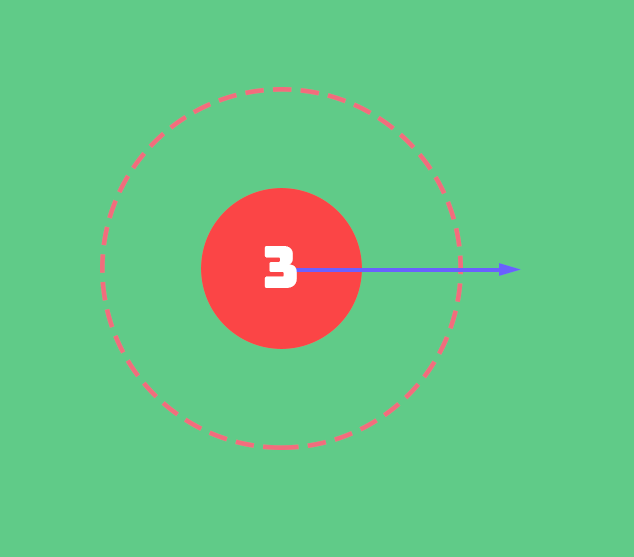
\includegraphics[height=5cm]{images/agent_V0.png}
				\caption{Prototype de la représentation graphique de l'agent en V0}
				\label{fig:agent0}
			\end{figure}
		
	}
	{
	Les agents et ces paramètres sont nécessaires pour lancer une simulation.
	}
	{
    On pourra lancer un match et vérifier que les joueurs aient bien un numéro, une équipe, une vitesse, une catégorie, une hitbox, une position, un score de récompense et une vitesse maximum. On peut afficher ces paramètres dans le terminal avec une fonction d'affichage telle que la fonction print().
    On implémentera un algorithme simple où un agent se déplace jusqu'au ballon et tire. On pourra vérifier cette intéraction à l'affichage.
	} 

 	\besoinVItem{Perception de l'agent}
	{
	 Par défaut  l'agent percevra ses alliés, la balle et les cages de but. C'est à dire que l'agent connaît à tout moment les positions des ses alliés, de la balle et des buts ennemis. On aura alors un vecteur :
	    $$
	 \begin{bmatrix}
	 	x\_agent & y\_agent & x\_allie\_agent & y\_allie\_agent \\
	 	x\_ball & y\_ball & x\_poteau1 & y\_poteau1 & x\_poteau2 & y\_poteau2 \\
	 \end{bmatrix}
	 \quad
	 $$
		
	}
	{	
		L'objet optionnel info retourné par env.step() de gym.OpenAI dans SlimVolleyGym permet de récupérer des infos sur l'opposant (il est donc facile de trouver les informations sur l'allié ou l'opposant ) :\\
		info = \\
		('ale.lives': agent's lives left,\\
		'ale.otherLives': opponent's lives left,\\
		'otherObs': opponent's observations,\\
		'state': agent's state (same as obs in state mode),\\
		'otherState': opponent's state (same as otherObs in state mode),)
		
	}
	{
	Pour entrainer et faire jouer l'agent on a besoin de lui donner une perception de l'environnement.
	}
	{
	Si l'agent arrive à intéragir avec la balle assez souvent on peut supposer qu'il la perçoit. On pourrait aussi adapter les fonctions de slime  pour simuler la vision de l'agent : test\_pixel.py. pour la vision pixel et test\_atari.py pour la vision par état (impact uniquement sur les réseaux de neuronne pour l'entraînement).
	} 

	\besoinVItem{Créer un équipe d'agent}
	{Une équipe doit être composée de 4 agents (pour l'instant), les agents d'une même équipe doivent pouvoir se reconnaître (se percevoir). Dans un match 2 équipes doivent s'affronter, pour les différencier on peut leur attribuer une couleur. L'équipe a un attribut score qui lui permet de garder le nombre de but marqué par l'équipe durant le match.}
	
	{On peut implémenter un agent dans slime donc il est possible de regrouper les agents en plusieurs groupes/équipes. On pense créer une classe équipe.}
	
	{Lorsque l'utilisateur lance le match, il verra les joueurs de l'équipe rouge à gauche du terrain et les bleus à droite. Le champ score de l'équipe est utilisé pour compter le score du match.}
	




	\besoinVItem{Caractéristiques du terrain}{
		Il est nécessaire de générer un terrain de foot conforme au règlement de la Robocup.
		Pour cela, il faut délimiter les différentes zones de jeux. Dans la V0 on aura une ligne pour représenter les buts, les limites du terrain (lignes de but et lignes de touche), la ligne médiane pour séparer le terrain en 2 et un point pour mettre la balle au centre. Les bords sont des murs qui empêchent les joueurs et le ballon de sortir du terrain.
		
	}
	{
		Le terrain est composé de formes géométriques simples comme des rectangles. On dispose de telles fonctions dans slimevolley comme la class Wall. 
		\begin{figure}[H]
			\centering
			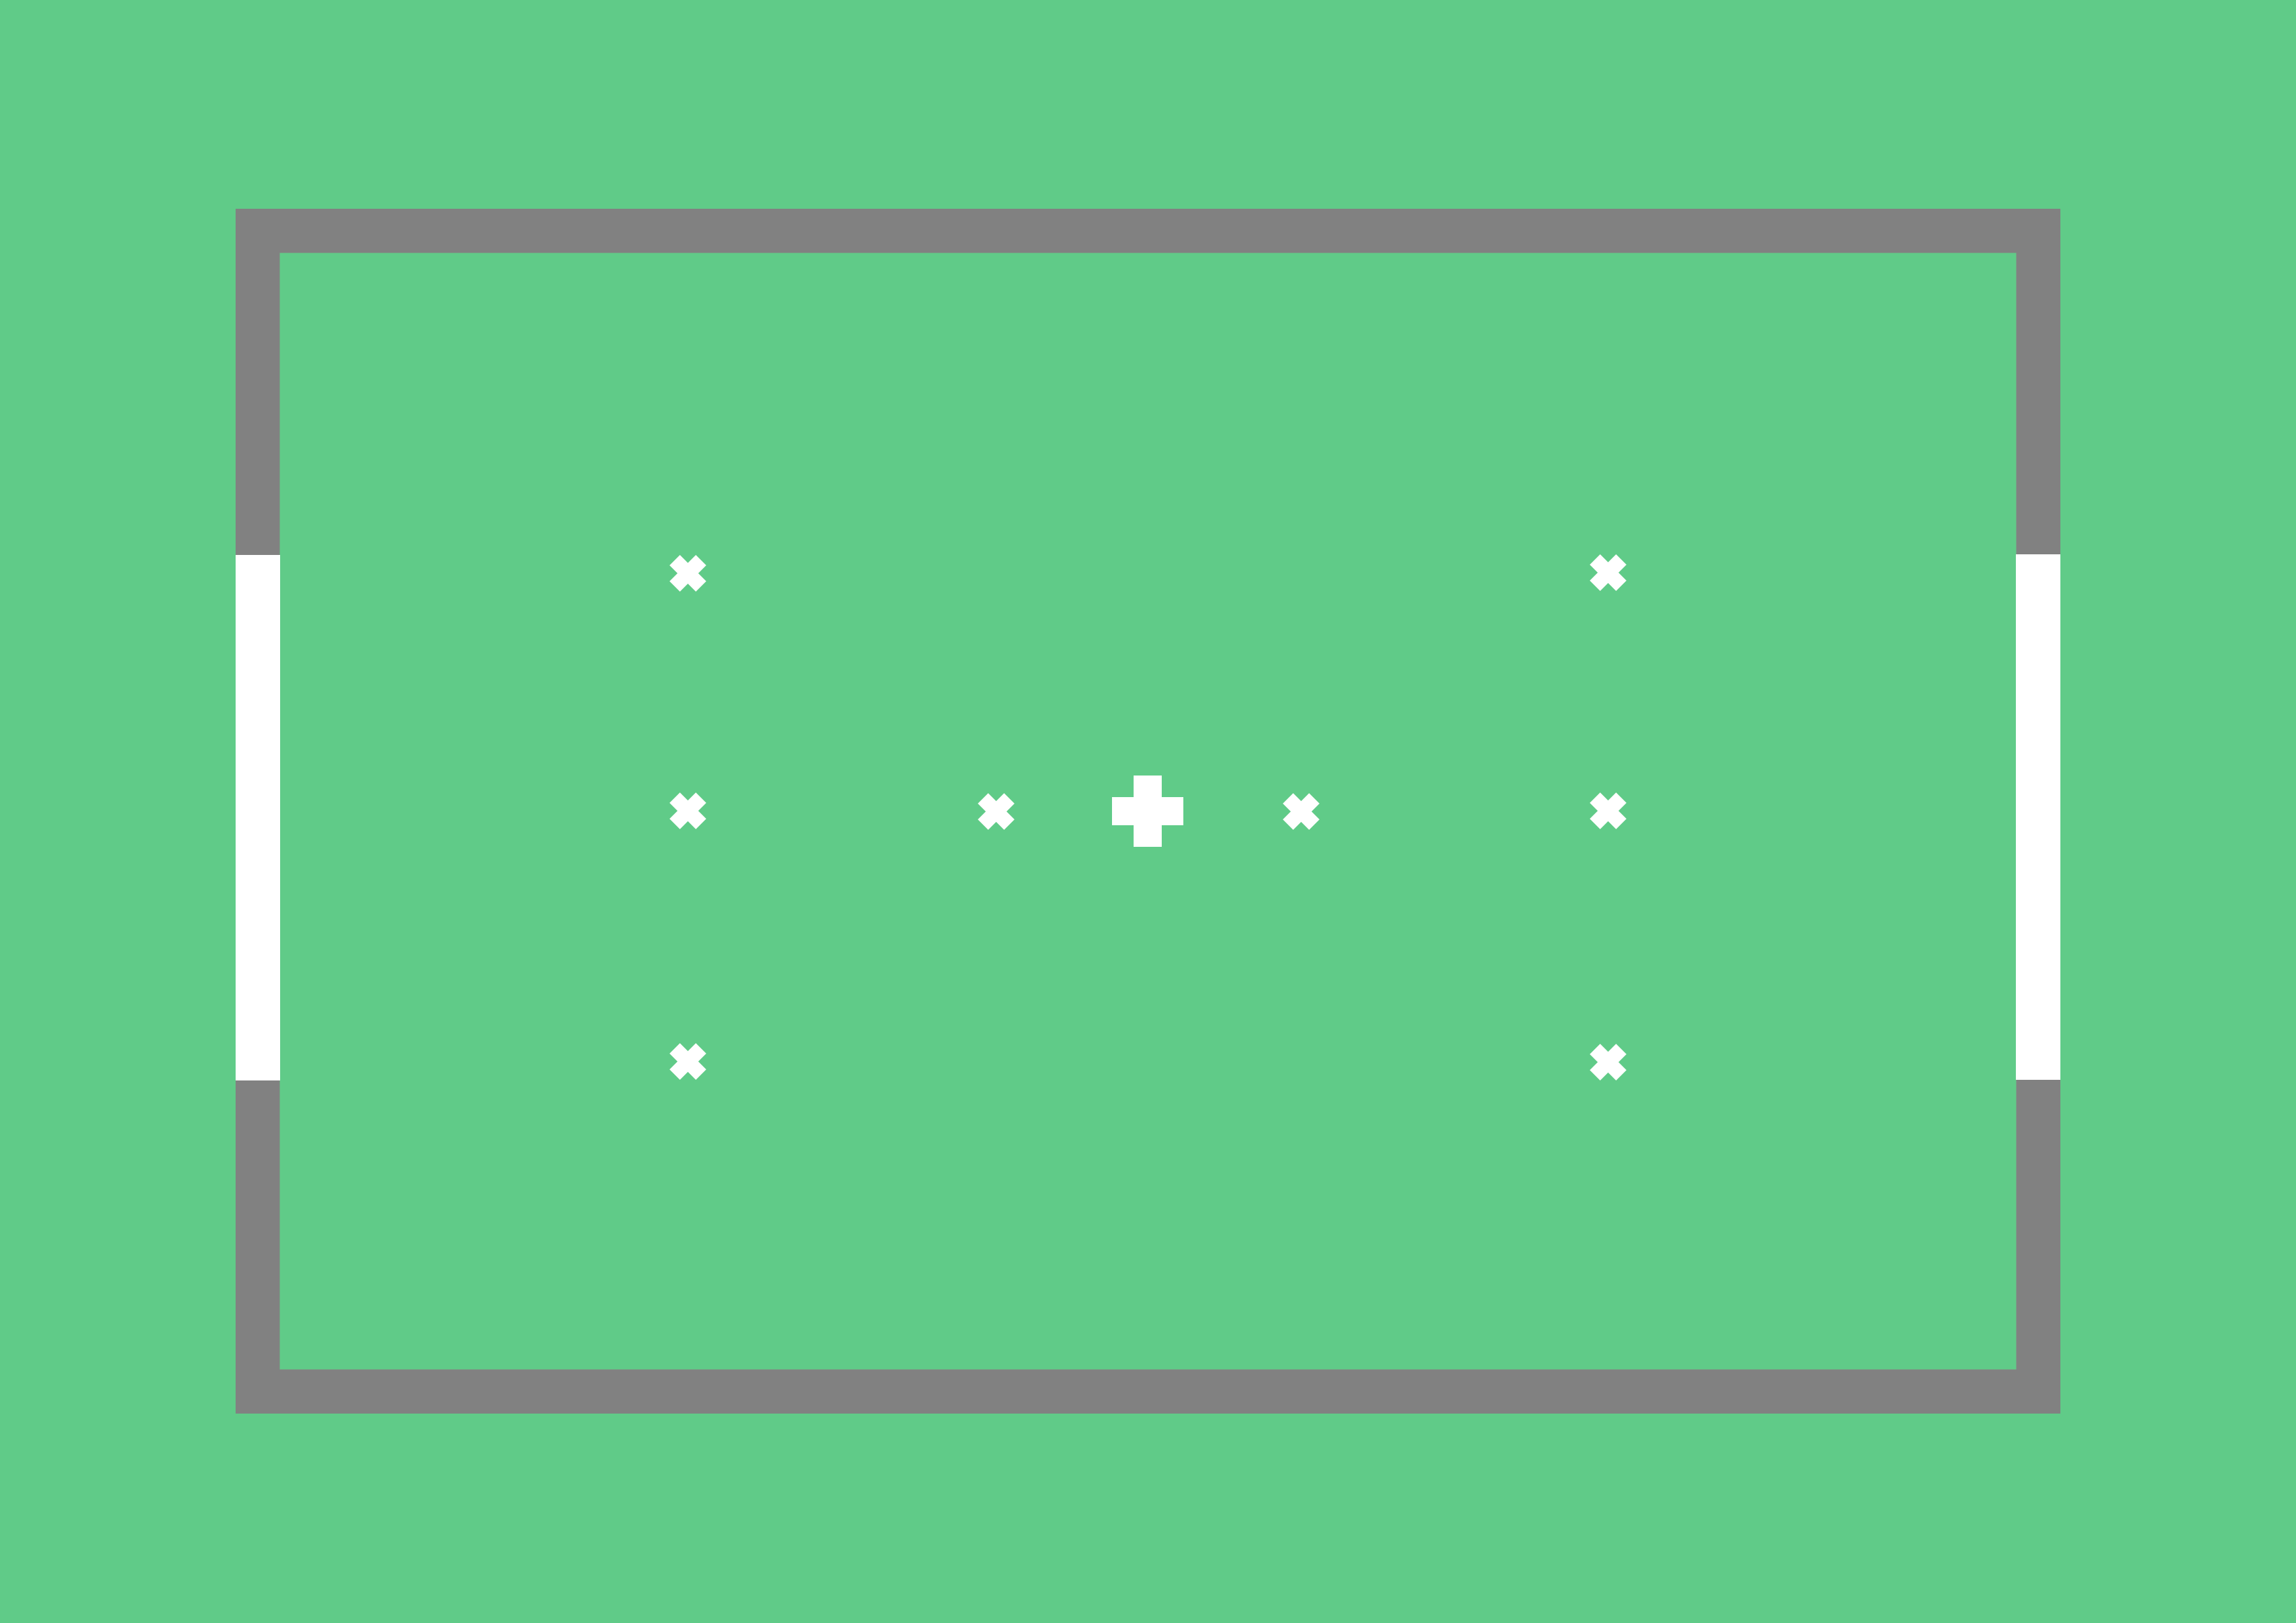
\includegraphics[height=5cm]{images/terrainV0.png}
			\caption{Prototype du terrain en V0}
			\label{fig:terrain0}
		\end{figure}
		
	}
	{
		On affiche un terrain : les déplacements du ballon et des joueurs sont limités à ce terrain. Le ballon doit pouvoir détecter la collision avec la ligne de but. Un agent ou le ballon peut tester la collision avec les limites du terrain.
		
	}
	{
		À l'affichage du match, regarder si on voit toutes les zones. Regarder les interactions de collision et vérifier qu'un but est bien marqué lorsque le ballon touche la ligne des buts.
	} 


	\besoinVItem{Caractéristiques de la balle }
		{	Il faut que le ballon soit simulé par un cercle qui réagit aux tirs et rebondit lors de collisions. 
		\begin{itemize}
			\item \textbf{Hitbox de la balle en forme de cercle} donnée avec le paramètre rayon.
			Pour simuler des collisions.
			\item \textbf{Position courante.} 
			C'est la position (x,y) de la balle sur le terrain à un instant donné.
			
			\item \textbf{Vitesse courante en vx et vy.} 
			C'est la vitesse de la balle à un instant donné.
			
			\item \textbf{Vitesse précédente en vx\_prec et vy\_prec.} 
			C'est la vitesse de la balle à un instant précédent donné.
		\end{itemize}
		}{
			Il est possible de vérifier la superposition de formes et changer le déplacement du ballon pour représenter le rebond, et de même pour le tir. 
			La classe Particle de Slimevolley implémente les fonctions checkEdges() bounce() et isColliding() et permet de gérer les interactions de la balle.
			
		}{La balle est nécessaire pour la simulation. 
		}{Lors d'un match, on vérifie si la balle apparaît et si elle peut bouger. }
		
	
		\besoinVItem{Déplacements de la balle}{
			Il faut simuler le déplacement du ballon pour que les joueurs et les limites du terrains puissent interagir avec la balle.
			
		}{
			Avant qu'un élément ait un impact sur la balle, il faut vérifier qu'il est en collision avec elle.
			Les déplacements sont implémentés avec les fonctions move(), applyAcceleration() et limitSpeed() dans le fichier slimevolley.py .\\
			move() v'=gamma*v pour l'accélération et v=a*timestep et pos=v*timestep
		}
		{Après un tir d'un agent, celui-ci donne une vitesse et une accélération. La fonction move() va ensuite déplacer le ballon à chaque tour de boucle de simulation.}
		
		{Il faut déplacer la balle, voir si elle s'arrête naturellement, si elle ne peut pas atteindre une vitesse trop rapide pour la simulation et voir si les éléments extérieurs ont un impact sur elle.}  
  
  	\besoinVItem{Déplacements de l'agent}
  
  {
  	Pour jouer au foot, les joueurs de la simulation devront se déplacer sur le terrain. On souhaite donc munir les joueurs d'une fonction de déplacement qui devra simuler le plus précisément possible les déplacements des robots de la RoboCup. Ces déplacements seront influencés par la vitesse et l'accélération du joueur.
  }
  {
  	Les déplacements sont implémentés dans SlimeVolleyGym dans le fichier slimevolley.py. On a une fonction move() qui permet de gérer les déplacements de l'agent, on pourra donc s'en inspirer.
  	Les déplacements possibles sont haut, bas, gauche, droite.
  }
  {
  	Lors de la simulation d'un match, un joueur va par exemple devoir s'approcher de la balle pour tirer. Il devra donc se déplacer jusqu'à la balle.
  }
  {
  	On peut vérifier les coordonnées du joueur avant et après déplacement afin de vérifier que le mouvement a bien eu lieu. Ou lancer la simulation et attendre qu'un agent bouge.
  } 


	\besoinVItem{Pouvoir tirer}
	{
		Pendant les matchs de la Robocup, les robots sont amenés à intéragir avec le ballon et notamment à tirer dedans. Dans notre simulation aussi les joueurs devront pouvoir tirer dans le ballon pour le déplacer. Il faudra donc munir les joueurs d'une fonction de tir. Le joueur effectuera une action qui propulsera le ballon dans une direction avec une vitesse et une accélération. 
	}
	{ Pour implémenter notre système de tir on pourra s'inspirer des fonctions iscolliding(), bounce() et setaction() de slimvolleygym.py. Il faudra donc gèrer la collision entre le joueur et la balle lors du tir, du rebond de la balle lorsqu'elle est propulsée, et de l'éxécution de l'action par le joueur.}
	{
	Fonctionnalité nécessaire pour déplacer la balle.
	}
	{
		En lançant un match, on pourra observer par moment les joueurs tirer dans le ballon (graphiquement, ou dans l'historique des actions du joueur) si la fonctionnalité est bien implémentée.
	} 

	\besoinVItem{Marquer un but} 
	{Les buts sont symbolisés par la ligne de but, c'est-à-dire que lorsque que la balle touche la ligne de but (au niveau des buts, pas toute la ligne), on considère que l'on vient de marquer. Si la balle rentre dans les cages bleues alors il y a but pour les rouges et inversement. Il faut modifier le score dès que la balle entre dans les cages.}
	
	{Comme dans slimevolleygym, la game doit vérifier elle même si elle est entrée en contact avec la ligne de but (collison). Lorsque c'est le cas le score de l'agent et de l'équipe est mis-à-jour en fonction. }
	
	{Utilisé pour gérer le déroulement du match.}
	
	{Mettre la balle dans les buts, voir si le score est mis à jour et si le match s'arrête.}
	
	
	\besoinVItem{Collision}
		{
		La collison est un moyen de vérifier si 2 éléments entrent en contact, ce cas est omniprésent dans notre projet. \\
  		Quand le ballon rebondit lors de collisions avec les murs et les agents. Il marque un but lors de collision avec la ligne de but.\\
    	La collision entre le ballon et la zone de tir de l'agent autorise la fonction de tir de l'agent.
	
		}
		{Faire comme dans smilevolley, il y a des fonctions de collisions (isColliding)}
		{On utilise la collision pour limiter et modifier le déplacement des agents et du ballon ainsi que pour marquer un but et tirer}
		{Vérifier tous les types de collisions en description}  

  \besoinVItem{Affichage}
	{
    Le terrain, les agents et le ballon sont des composants visibles. L'objet Game assure un affichage actualisé en appelant la fonction d'affichage de chaque agent du ballon et du terrain. Le game affiche le temps au dessus du terrain.
	}	
	{On aura des fonctions display pour chaque éléments comme dans SlimeVolley. Comme par exemple def display(self, canvas, bx, by)}
	{Lancer un match ouvre une fenêtre ou l'on peut observer le déroulement du match}
	{On vérifie qu'il y a un affichage et qu'il représente le jeu sans erreur. On affiche dans la fenêtre une donnée et on regarde la même donnée s'afficher dans le terminal pour comparer.}  


\end{enumerate}
\subsubsection{Robocup version 1 (V1)}

Cette version est paramétrable. Le déroulement du jeu a changé puisque maintenant le match de 10min et ne s'arrête pas en cas de but.
Voici une liste des options :
	\begin{itemize}
		\item taille du terrain : Kid/Adult
		\item taille des agents : Kid/adult
		\item orientation des agents : on/off
		\item Nombre d'agents dans une équipe (2-5)
		\item Fautes on/off si activé choisir parmi : touche/exclusion/les deux
		\item collision entre agents on/off
		\item placement libre on/off
	
		
	\end{itemize}
\begin{enumerate}
	
	\besoinVItem{Organiser un match}
	{ Dans cette version du jeu, le placement initiale est libre. Le Game va maintenant avoir des fonctions supplémentaires à réaliser. Il va exclure les joueurs s’il le faut, gérer les touches et les fautes. Le match s’arrête à 10min avec une inversion des cotés à 5min de jeu. Marquer un but n’est plus une condition d’arrêt mais déclenche un engagement.}
	{trivial}
	{C’est le besoin qui met en lien tout les autres. On permet de lancer et organiser des matchs.}
	{On vérifie la nouvelle durée du match et qu'il lance les phases de jeu dans le bon ordre. Il faut que les autres besoins fonctionnent pour pouvoir finalement lancer une partie entièrement fonctionnelle.}


	\besoinVItem{Caractéristiques d'un joueur/agent}
	{ 
		
		\begin{itemize}

			
			\item Attribuer une orientation au joueur, si ce paramètre est activé alors il faut modifier la hitbox de tir. On a décidé d'opter pour un demi-cercle. On rajoute des yeux à l'agent pour montrer son orientation (affichage).
			
			\item Catégorie de joueur : KidSize ou AdultSize, en adult la hitbox des agents est plus grande.
			
			\item immobilisé (booléen) ce champ varie au cours de la partie. Au début il est à false mais si le joueur est exclu, il passe à true et celui-ci ne peut plus se déplacer et tirer.

	
		\end{itemize}
	}
	{
		Changer les hitbox des agents dans les paramètres avant l'initialisation.  
		\begin{figure}[H]
			\centering
			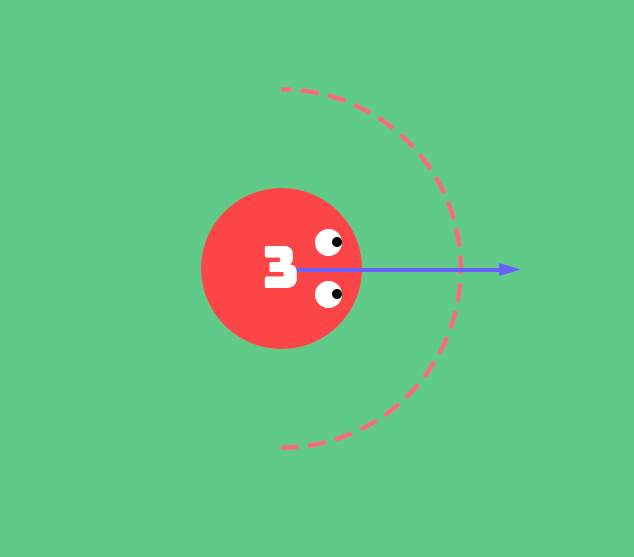
\includegraphics[height=5cm]{images/agent_V1.png}
			\caption{Prototype de la représentation graphique de l'agent en V1}
			\label{fig:agent1}
		\end{figure}
		
	}
	{
	Dans les paramètres, l'utilisateur peut choisir l'orientation de l'agent, et sa catégorie.
	}
	{
		Tester si les différentes catégories changent bien l'environnement, vérifier que les agents ne tirent pas de dos avec orientation activée.
	} 

	\besoinVItem{Ajouter un champ last-touched }
	{On veut rajouter un paramètre sur la balle qui stocke la dernière équipe à avoir touché la balle.  }
	
	{On donne une couleur à la balle en fonction de la dernière équipe qui a touché la balle et la change dès qu'un joueur d'une autre équipe la frappe. On pourra afficher la balle de la couleur de la dernière équipe qui l'a touchée.}
	
	{On pourra utiliser ce champ pour les touches et déterminer qui a fait une faute. }
	
	{Vérifier que la balle prend la bonne couleur pendant les différents tirs.}
	
	
	\besoinVItem{Zones de terrain manquantes}
	{ Le terrain est maintenant complet avec 2 tailles disponibles :kidSize et adultSize voir les dimensions en figure\ref{fig:dim_ter}.
		Il faut rajouter les zones : 
	\begin{itemize}
		\item ligne médiane
		\item surface de réparation
		\item zone de but
		\item zone d'engagement
		\item cages
		\item zone d'exclusion
	\end{itemize}

		\begin{figure}[H]
		\centering
		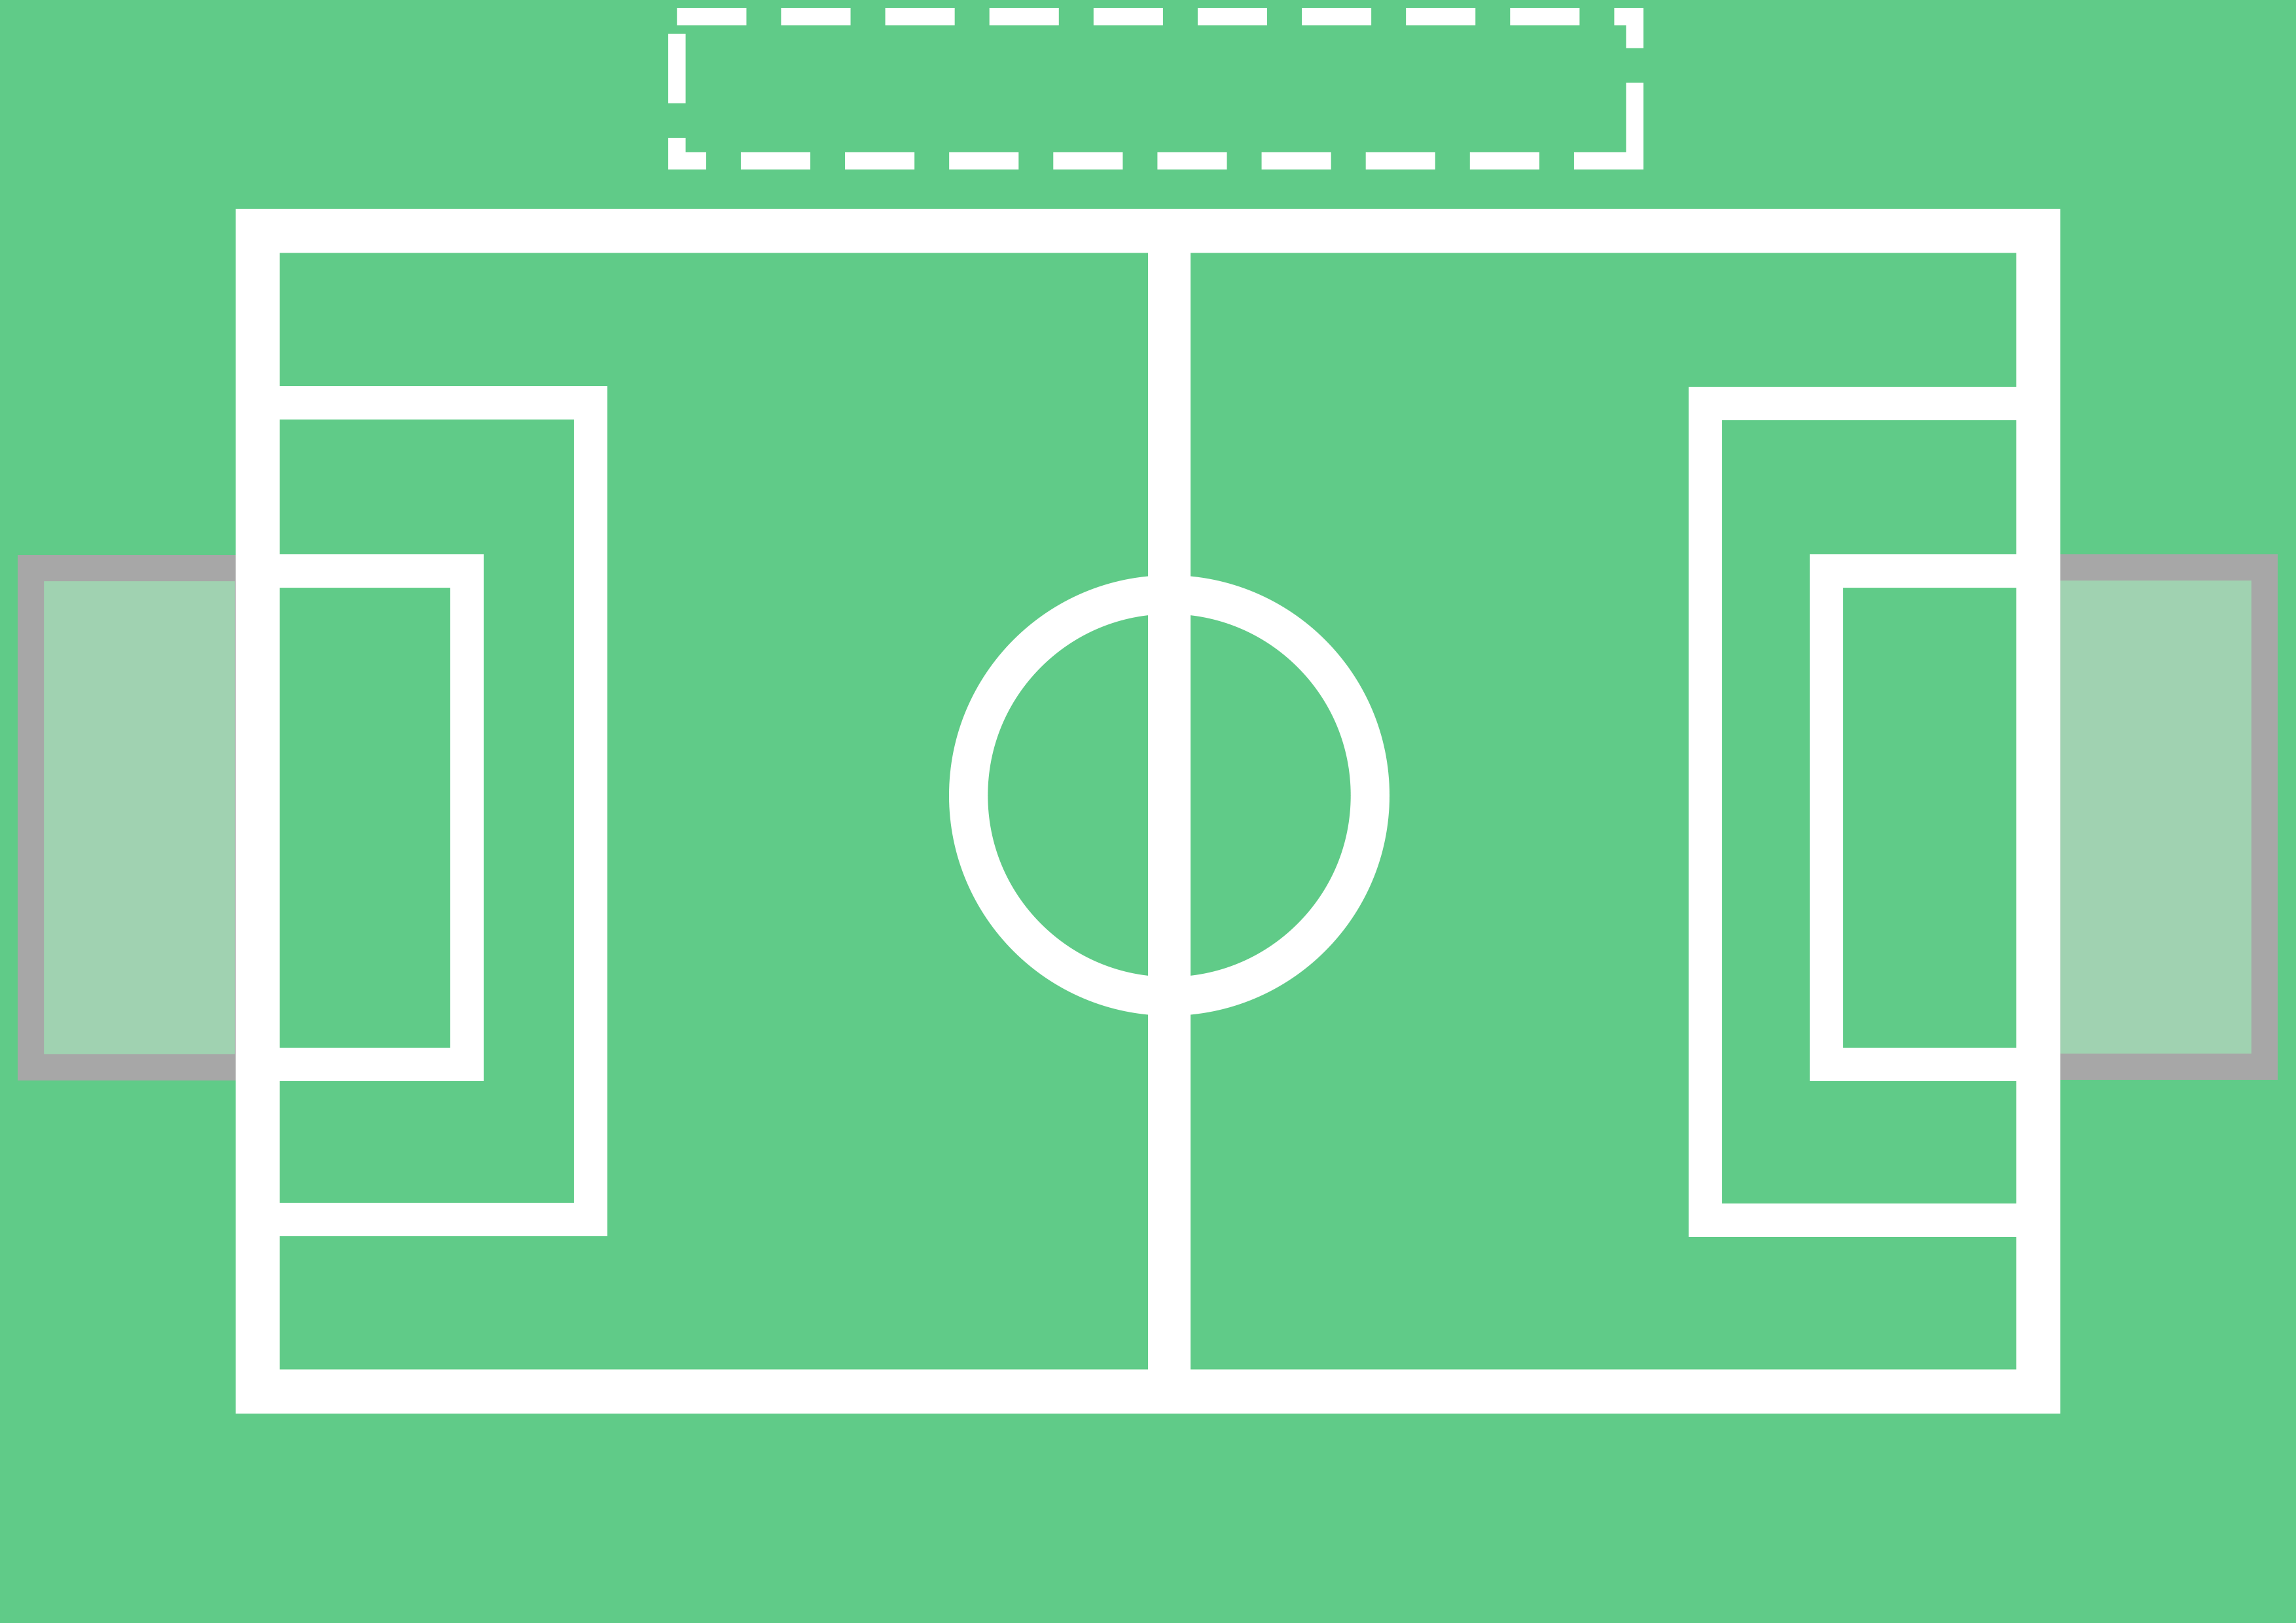
\includegraphics[height=5cm]{images/TerrainV1.png}
		\caption{Représentation graphique du terrain en V1}
		\label{fig:terrain1}
	\end{figure}


	}
	{Pour faire les différentes zones on peut créer un objet correspondant à chaque zone (même principe que la class Wall dans SlimeVOlleyGym).}
	{ Ces zones sont nécessaires pour la réalité de la simulation, elle seront utiles dans les versions futures.}
	{Pour tester il faut lancer un match et vérifier que toutes les zones sont visibles.}

 	\besoinVItem{Choisir le nombre de joueurs}
	 {On doit pouvoir choisir le nombre d'agent dans une équipe, pour l'instant entre 2 et 5 joueurs.}
	 {Il faut rajouter un paramètre qui permet de choisir la taille de l'équipe et initialiser l'équipe puis les agents à partir de là.}
	 {Le nombre de joueur permet de faire varier l'environnement et les stratégies qui seront mise en place.}
	 {Lancer un match avec toutes les tailles d'équipe et vérifier que le compte y est.}
	 
	 \besoinVItem{Nouvelle phase de jeu : l'Engagement}
	 {Le match débute par l'engagement, la balle doit être placée au centre du terrain, l'équipe qui n'engage pas doit être à une certaine distance de la balle (0.75m en kid 1.5m en adult). Chaque équipe doit être dans sa moitié de terrain. Le chrono du match est lancé une fois que la balle est en mouvement ou au bout de 10s. Après un but il y a une phase d'engagement la balle est pour l'équipe qui vient d'encaisser le but. On pourrait dire qu'à la première mi-temps la balle est pour les bleu et à la deuxième elle est pour les rouge.}
	 {Pour la phase d'engagement on peut s'inspirer de la fonction newMatch de slimevolleyGym qui remet la balle en jeu quand un point à était marqué. }
	 {Lorsque l'utilisateur lance un match/mi-temps celui-ci débute par un engagement. Il y a aussi engagement après un but. }
	 {Vérifier au lancement du match que les règles de placement sont respectées, que si personne ne tir, le chrono se lance au bout de 10s et qu'à chaque mi-temps l'équipe qui engage n'est pas la même. Vérifier qu'après un but la bonne équipe engage.}
	 
	 \besoinVItem{Placement des joueurs libres}
	 {On peut choisir d'activer le placement imposé de la V0 mais maintenant on peut laisser les agents se placer là où ils le souhaitent. Si un des agents ne respecte pas les règles de l'engagement (placement, attente, ..) alors il est exclu temporairement(le temps du lancement du match). }
	 {Si on veut utiliser le placement de V0, il faut l'adapter pour 2,3,5 joueurs.\\
	 	Pour le placement libre, il faut exclure les joueurs avec la fonction d'exclusion. }
	 {Le placement des joueurs est nécessaire au début de chaque phase de jeu.}
	 {Vérifier si les joueurs mal placés sont exclus, vérifier qu'ils peuvent revenir sur le terrain et ne restent pas bloqués à l'extérieur. }
	
	\besoinVItem{Collisions entre agents }
	{Dans cette version on veut pouvoir activer les collisions entre agents. Pour l'instant on active la collision uniquement entre adversaires. }
	{On se sert de la hitbox des agents et on crée une nouvelle fonction collision qu'il faudra vérifier dans la Game. Il faut regarder le champ équipe pour la collision, si les agents sont dans la même équipe il ne se passe rien.}
	{On va utiliser les collisions entre agents pour simuler les fautes.}
	{On regarde si la collision entre 2 agent provoque des événements.}
	
	\besoinVItem{Exclusion du terrain}
	{S'il y a collision, il y a faute. Si l'agent et mal placé ou ne respecte pas les temps d'arrêt, il commet une erreur. Après une faute ou une erreur, on peut exclure les joueurs impliqués pendant 10s. Pour cela, il faut créer une zone pour revenir sur le terrain. Cette zone est située sur la zone médiane, les joueurs exclus d'une équipe rentrent chacun d'un coté.
	 }
	{Pour exclure le joueur, il faut regarder s'il est entré en collision avec un adversaire, s'il est mal placé ou s'il bouge pendant un arrêt de jeu. Si oui, on passe son champ immobilisé à true, ce qui a pour effet de l'empêcher de bouger et de tirer. On le téléporte à l'extérieur du terrain sur sa zone d'entrée. Une fois sa pénalité écoulée, on passe son champ immobilisé à false.\\}
	{Les fautes et erreurs sont utiles pour modifier l'environnement. Elles sont désactivables. L'exclusion permet de nouvelles stratégies, on pourrait penser dans le futur à prendre en compte les temps d'exclusion pour l'apprentissage.}
	{Vérifier le bon déroulement d'une faute.}
	
	\besoinVItem{Touche}
	{Lorsque le ballon sort du terrain. L’équipe qui n’est pas celle de l’attribut Last\_touched du ballon envoie un joueur derrière qui reste à l’endroit de la touche. Le joueur est avant autorisé à sortir du terrain. Il peux ensuite tirer à un angle entre 0 et 180 degré ( ce qui est normal vu la position de l’agent) . Une fois qu’il a tiré, il a 5s pour retourner sur le terrain avant de perdre son immunité aux sorties de terrain   }
	{On fait appelle à des fonctions déjà décrites comme tirer et se déplacer}
	{Cette phase de jeu implémente les règles de la robocup lors d’une sortie de ballon}
	{En jouant une partie, on tire le ballon en dehors des démarcations et on vérifie que la phase de touche se déroule comme dans la description.}

\end{enumerate}

\subsubsection{Robocup version 2 (V2)}
	Notre priorité est de fournir les V0 et V1 de l'application. C'est pourquoi les besoins que nous nous proposons d'implémenter dans cette version seront plus susceptibles d'être modifiés en fonction des contraintes que nous rencontrerons lors du développement.
	Cette version permettra probablement des intéractions plus complexes entre les agents et leur environnement. 
	Voici une liste des options supplémentaires qui seront potentiellement présentes dans cette V2 :

	\begin{itemize}
		\item \textbf{Hitbox carrée pour les joueurs.} on pourrait imaginer d'autres formes si cela a un intêret : ellipses, rectangles ...\\
		\item \textbf{Hitbox en forme de cône pour le tir.} Comme pour la hitbox de l'agent, on pourrait fournir une portée customisable pour le tir  par l'utilisateur.\\
		\item \textbf{Activer l'herbe.} La balle subirait une action ralentissante de l'herbe lorsqu'elle roule à contre-sens des brins.\\
		\item \textbf{Champ de vision paramètrable pour les joueurs.} Les agents auraient accès aux informations sur l'environnement dans un arc de cercle de taille paramètrable devant eux.\\
		\item \textbf{Système de chute.} Si un agent entre en collision avec un autre agent (allié/ennemi) ou un poteau, on simulerait sa chute : il serait immobilisé le temps qu'il se relève. On pourrait aussi simuler la chute après certains tirs.\\
		\item \textbf{Fonctions de tir différentes} en fonction de la size (modification de la force), ainsi qu'un tir pied droit et un tir pied gauche.\\
		\item \textbf{Tailles d'équipe déséquilibrées.} (4v5, 2v6 ...etc)\\
		\item \textbf{Pouvoir paramètrer le temps d'exclusion lors de pénalité.}\\
		\item \textbf{Réussir à déterminer quel agent est sanctionné lorsqu'une faute a lieu.} La faute sera probablement attribuée à l'agent le plus éloigné de la balle.\\
		\item \textbf{Implémentation des coups francs et penalty.} \\
		\item \textbf{Laisser à l'IA choisir le positionnement au début des phases de jeu.} (début du match/après un but). Gestion de pénalité au cas où l'agent sortirait du terrain.\\
		\item \textbf{Pouvoir modifier la zone de rentrée des agents sur le terrain après une exclusion.}\\
		\item \textbf{Influence des exclusions sur l'attribut reward de l'agent.}
		
\end{itemize}
		


\subsection{Besoins communs entre toutes les versions de la Robocup}
\begin{enumerate}
  \besoinItem{Pouvoir lancer un match avec des IA qui s'affrontent }{On souhaite pouvoir faire s'affronter deux IA (pas forcément différentes) l'une contre l'autre lors d'un match simple et dans un environnement prédéfini.}
  {\textit{Mandatory}}
  {Dans la version initiale de slimeVolleyGym, on peut choisir l'IA que l'on veut utiliser en ligne de commande, avec --left ou --right. On peut reprendre ce principe pour soit l'implémenter dans un fichier JSON, soit l'implémenter à l'aide d'une CLI. Comme défini dans le besoin fonctionnel du chapitre 3.4.1.}
  {SlimevolleyGym }
  {Chaque fois que l'utilisateur voudra entrainer ou tester une IA, il devra utiliser cette fonctionnalité. Il choisira quelles IA s'affronteront en ligne de commande.}
  {Pour tester la simulation, nous pouvons utiliser un algorithme qui prend des décisions aléatoires et vérifier que des décisions ainsi que des actions sont effectué lors d'une partie.}	
  
  \besoinItem{Pouvoir entraîner un agent/équipe sur la simulation}
  {On souhaite pouvoir utiliser un algorithme d'apprentissage par renforcement pour entraîner un/plusieurs agents (d'une même équipe) dans un environnement prédéfini et avec un nombre de match fixé. }
  {\textit{Mandatory}}
  {Pour cela on utilise la bibliothèque Gym qui a des fonctions spécifique qui gèrent l'espace d'observation et l'espace d'action des agents, on peut aussi mettre en place un système de récompense. On prendra exemple sur slimevolleygym qui utilise déjà la bibliothèque gym pour entrainer des agents suivant différent algorithme dans différents environnement.}
  {SlimevolleyGym et Gym}
  {Une fois l'algorithme choisit par l'utilisateur ainsi que son nombre d'essais, son adversaire et son environnement. La ligne de commande associé va permettre de lancer en tâche de fond(sans visuel), un match entre l'algorithme de l'utilisateur et l'algorithme adverse(il peut jouer contre lui-même) un nombre choisit de match.}
  {On créer un algorithme basique (son but est de courir jusqu'à la balle, de s'aligner et de tirer vers les cages adverse) qui va s'entraîner contre un algorithme aléatoire. On vérifie à la fin que la différence de point entre le nombre de point marqué par les deux algorithmes est de plus en plus positive. Ce qui signifie que notre algorithme à marqué plus de but ou s'en est moins prit.}
  
  \besoinItem{Pouvoir enregistrer une IA entrainée}
  {Après avoir entrainée une IA il faut pouvoir enregistrer le résultat pour pouvoir la comparer sans à chaque fois devoir la ré-entrainer.}
  {\textit{Mandatory}}
  {Lorsque l'on est en mode entrainement on enregistre automatiquement l'apprentissage sur l'IA entrainée. }
  {}
  {Après un entrainement satisfaisant on enregistre l'IA. utile pour comparer plusieurs version entrainer dans différent environnements.}
  {Entrainer une IA, l'enregistrer, quitter l'entrainement et voir si on peut lancer un match avec le résultat de l'entrainement.}
  
   \besoinItem{Avoir des IA basiques pour tester de lancer des matchs et vérifier leur bon fonctionnement}
   { Pour pouvoir tester les fonctionnalités de notre simulation, il nous faut des algorithmes basiques tel que random ou "je cours vers la balle et dès que je l'ai, je tire en direction du but" }
  {\textit{Mandatory}}
  {Des algorithmes simples sont déjà implémenté dans slimevolleygym. Nous pouvons les adapter pour qu'ils puissent intégrer les nouvelles dimensions de la version RoboCup.}
  { faire un lien vers les fichiers de test de slimevolley}
  {L'utilisateur peut lancer un match de test en sélectionnant un algorithme déjà entraîné qui jouera contre lui-même ou un joueur random suivant le chois de l'utilisateur.}
  {On lance un match, avec les algorithmes et on observe leur gameplay.}
  
  \besoinItem{Faire un mode test et un mode entraînement}
  {Il faut pouvoir lancer des matchs pour faire des tests sans que les IA progressent en jouant pour une meilleure comparaison des résultats.}
  {\textit{Mandatory}}
  {On aura un script d'entrainement et de test, on pourra appeler l'IA que nous souhaitons entrainer et contre qui en option de commande sur le fichier train. Même fonctionnement pour les tests. On s'inspirera de SlimeVolleyGym pour les script. }
  {SlimeVolleyGym }
  {Pour comparer l'impact des environnements sur les IA (leur entrainement) il faut faire des tests sur plusieurs match. Si les IA évoluent en phase de test on risque d'avoir des résultats biaisés.}
  {Lancer des match de tests dans un environnement défavorable à une des IA et voir si elle jouent de la même manière au début et à la fin.}
  
   \besoinItem{Pouvoir enregistrer les paramètres d'un environnement}{Après avoir sélectionner nos paramètre il peut être intéressant de les enregistrer pour éviter de les sélectionner à plusieurs reprise.}
   {\textit{Optionnal}}
   {Il faudra sauvegarder le fichier de paramètre JSON et rajouter une option en ligne de commande pour pouvoir lancer des tests ou des entrainements avec un fichier de paramètre en option.}
   {}
   {Cette fonctionnalité peut être pratique pour l'utilisateur qui n'aura pas à sélectionner les paramètres au début de chaque match.}
   {Lancer un match avec des paramètre enregistré vérifier si les paramètres choisis sont les bon et pas ceux par défaut.}
   
   \besoinItem{Déterminer un gagant/perdant/nul}
   {Pour obtenir des statistiques sur les tests (principalement qui a gagné contre qui dans quel environnement)il faut pouvoir déterminer un gagnant.}
   {\textit{Optionnal}}
   {Pour savoir qui est le gagnant il faut regarder le score du match qui sera dans le champ score de chaque équipe. L'équipe qui à le meilleur score gagne, il suffit de vérifier qui est le gagnant une fois que le match est fini. }
   {}
   {On pourrait afficher le gagnant du match à la fin. Cette information peut être utile pour faire des statistique mais ce n'est pas une priorité on peut aussi trouver le gagnant en comparant les scores à l'analyse.}
   {Regarder à la fin du match si le nom de l'équipe gagnante apparait.}
   
     
   \besoinItem{Avoir un menu pour choisir les paramètres du match}
   {Avoir une interface graphique avec les options à sélectionner en cliquant.  }{\textit{Optionnal}}
   {Ce besoin est en option et est loin d'être prioritaire, nous n'aurons probablement pas assez de temps pour l'implémenter.}
   {}
   {Cela permettrait de donner une meilleur visibilité des options choisies, de plus on pourrait modifier une option choisie au début si l'on s'été trompé et l'utilisateur aurait juste besoin de cliquer.}
   {Lancer ue partie et voir si le menu s'affiche et s'il fonctionne.}
  
\end{enumerate}
\subsection{Besoins Non-fonctionnels}
Notre sujet étant une demande d'application basée sur le modèle de SlimeVolleyGym, nous n'avons pas eu à penser la partie contrainte des performances ni à trop se pencher sur l'architecture du code à implémenter. Nous savons où nous devons aller, quelles bibliothèques, et quels algorithmes d'IA  utiliser. Normalement nous ne devrions pas avoir trop de surprises en passant à l'implémentation. Les enjeux du projet étaient surtout de comprendre le code et l'intérêt de SlimeVolleyGym pour la simulation Robocup, fournir un modèle qui utilise l'apprentissage par renforcement sans rentrer dans les détails, réussir à structurer et limiter les possibilités d'options. 

L'unique besoin non-fonctionnel serait dû à la richesse de la simulation, c'est-à-dire que l'apprentissage pourrait être très long sur un environnement trop complexe, mais notre version sera paramétrable et il sera possible de débuter l'entraînement avec le minimum d'informations. 

De plus notre client a été raisonnable et ne nous a pas fait de demandes incongrues. C'est pourquoi nous n'avons pas de besoins non-fonctionnels à présenter.

\section{Logiciels et architecture}


\section{Défauts et bugs}
Nous pourrions avoir des problèmes de compatibilité des options. Pour cela il va falloir faire de nombreux tests. 
Nous devons aussi nous assurer que les fonctions que nous réutiliseront de SlimeVolleyGym fonctionneront correctement sur la Robocup. 


\section{Diagramme de Gantt}
\begin{figure}[H]
    \centering
    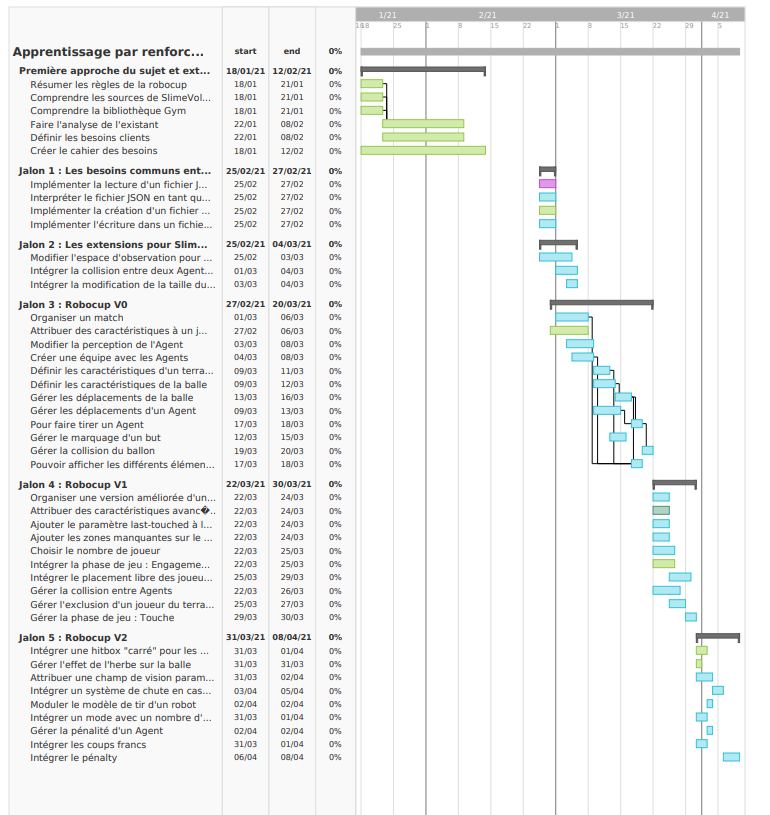
\includegraphics[scale=0.75]{images/GANTT.PNG}
    \caption {Diagramme de GANTT prévisionnel du projet}
\end{figure}

\section{Bibliographie}

\bibliographystyle{elsarticle-num}
\bibliography{Sources}


\end{document}
